\documentclass[12pt,a4paper]{article}

% ── Packages ─────────────────────────────────────────────────────────────────
\usepackage[a4paper, margin=2.5cm]{geometry}
\usepackage{amsmath, amssymb}
\usepackage{graphicx}
\usepackage{booktabs}
\usepackage{array}
\usepackage{caption}
\usepackage{subcaption}
\usepackage[colorlinks=true, linkcolor=blue!60!black,
            citecolor=blue!60!black, urlcolor=blue!60!black]{hyperref}
\usepackage[ruled, linesnumbered, noend]{algorithm2e}
\usepackage{listings}
\usepackage{xcolor}
\usepackage{parskip}
\usepackage{microtype}
\usepackage{float}

% ── Code listing style ────────────────────────────────────────────────────────
\lstdefinestyle{pycode}{
  language=Python,
  basicstyle=\ttfamily\small,
  keywordstyle=\color{blue!70!black}\bfseries,
  commentstyle=\color{gray},
  stringstyle=\color{orange!70!black},
  numberstyle=\tiny\color{gray},
  numbers=left,
  numbersep=8pt,
  frame=single,
  framerule=0.4pt,
  rulecolor=\color{gray!40},
  backgroundcolor=\color{gray!5},
  breaklines=true,
  showstringspaces=false,
  tabsize=4,
  xleftmargin=1.5em,
  xrightmargin=0.5em,
  captionpos=b,
}
\lstset{style=pycode}

% ── Title ─────────────────────────────────────────────────────────────────────
\title{%
\begin{spacing}
	\begin{center}
		\includegraphics[scale = 0.45]{figures/iut_logo.png}
		%Two images here for University of Warwick students, the colour crest and the black and white crest. Replace as appropriate!
	\end{center}
	\vspace{5mm}
	\begin{center}
		\textbf{\begin{LARGE}
		ISLAMIC UNIVERSITY OF TECHNOLOGY
		\end{LARGE}}
		\vspace{5mm}
	\end{center}
	\begin{center}
		{\large CSE 4733: Digital Image Processing}\\
		\vspace{20mm}
	\end{center}
	\begin{center}
		{\textbf{\begin{LARGE}
		    Tutorial Note on Generalized Hough Transform
		\end{LARGE} }}
		\vspace{20mm}
	\end{center}
	\begin{center}
	     {\large Name: Mehreen Hossain Chowdhury }\\
		{\large  ID: 210041219}\\
		{\large Section: 2A}\\
		{\large Department: CSE\\}
            \vspace{5mm}
            {\large Date of submission: 29th March, 2026\\}
	\end{center}
\end{spacing}
}

% ─────────────────────────────────────────────────────────────────────────────
\begin{document}
\date{}
\maketitle
\hrule
\vspace{1.2em}

% ── Abstract ─────────────────────────────────────────────────────────────────
\begin{abstract}
In this tutorial note, we present the Generalized Hough Transform (GHT), introduced by
Dana~H. Ballard in his 1981 paper \textit{``Generalizing the Hough Transform to
Detect Arbitrary Shapes.''}  The classical Hough Transform is limited to shapes
expressible by a closed-form parametric equation.  Ballard's generalization replaces
that equation with a precomputed look-up table, named the \textit{R--table}, which encodes
the spatial relationship between boundary points of an arbitrary template shape and a
chosen interior reference point, indexed by local gradient orientation.  This note
describes the working principle of the GHT, derives the formal algorithm, presents
pseudocode, traces step-by-step execution on real images, and provides an in-depth experimental analysis on real images.
\end{abstract}

\tableofcontents
\newpage

% ═════════════════════════════════════════════════════════════════════════════
\section{Introduction}
% ═════════════════════════════════════════════════════════════════════════════

Identifying specific shapes remains a fundamental challenge within computer vision. Fields like industrial quality control, medical diagnostics, and document processing frequently require pinpointing geometrically intricate target objects within an image. For mathematically definable shapes like lines or circles, the traditional Hough Transform~\cite{hough1962} offers a refined approach by treating the detection process as a voting mechanism within a parameter space. Duda and Hart~\cite{duda1972} popularized the $(\rho, \theta)$ parameterization for lines; adapting the method for circles requires an additional radius dimension, while expanding it to ellipses necessitates a five-dimensional space. The primary drawback to this method is the strict requirement of deriving a distinct parametric equation for every new shape class.

While an earlier technique developed by Merlin and Farber~\cite{merlin1975} could process non-analytic curves, it was strictly limited to translational shifts. Ballard~\cite{ballard1981} significantly expanded this framework to accommodate arbitrary shapes \emph{and} variations in rotation and scale, thereby transforming the algorithm into a highly versatile tool. The underlying premise is that the boundary of any shape, no matter how complex, can be mapped by grouping the displacement vectors from the edge pixels to an internal reference point based on their local gradient orientation. This collection of vectors, known as the R--table, is generated directly from a single template image, completely eliminating the need for any analytic description.

This tutorial is structured as follows.  Section~\ref{sec:background} reviews the
classical Hough Transform.  Section~\ref{sec:algorithm} develops the GHT formally.
Section~\ref{sec:pseudocode} states the algorithm as pseudocode.
Section~\ref{sec:scale_rotation} covers the scale and rotation extensions.
Section~\ref{sec:worked} traces a complete step-by-step worked example on real images.
Section~\ref{sec:results} presents results on multiple real images.
Section~\ref{sec:analysis} gives an in-depth experimental analysis.
Section~\ref{sec:conclusion} concludes.

% ═════════════════════════════════════════════════════════════════════════════
\section{Background: The Classical Hough Transform}
\label{sec:background}
% ═════════════════════════════════════════════════════════════════════════════

\subsection{Voting in Parameter Space}

Hough Transform recasts the problem of finding a shape in image
space as one of finding a peak in a parameter space.  Every edge pixel $(x, y)$ is
treated as a constraint: it emits a vote for every parameter combination that would
place a curve of the target shape through that pixel.  When enough edge pixels agree
on a common parameter set, a peak emerges in the accumulator and signals a detection.
For a line expressed as $\rho = x\cos\theta + y\sin\theta$, each pixel votes along a
sinusoidal curve in $(\rho, \theta)$ space.  Detecting a circle
$(x-a)^2 + (y-b)^2 = r^2$ requires a three-dimensional accumulator over $(a, b, r)$. As the votes are cast independently, noise,
clutter, and partial occlusion degrade peak height gradually rather than breaking
detection outright.  The cost is that the accumulator must be parameterised in a form
that matches the target shape exactly.

\subsection{Where the Classical Transform Falls Short}

Every shape class demands a fresh parameterisation.  Circles need one formula,
ellipses need another, and most real-world objects like tool parts, anatomical
structures, printed characters do not correspond to any convenient closed form at
all.  This is the gap that Ballard's extension was designed to fill.
Table~\ref{tab:comparison} summarises how the two approaches compare across the
properties most relevant in practice.

\begin{table}[H]
\centering
\caption{Comparison of the Classical and Generalised Hough Transforms.}
\label{tab:comparison}
\renewcommand{\arraystretch}{1.3}
\begin{tabular}{@{} l p{5cm} p{5cm} @{}}
\toprule
\textbf{Property} & \textbf{Classical HT} & \textbf{Generalised HT} \\
\midrule
Shape class        & Lines, circles, conics only & Any arbitrary closed shape \\
Shape description  & Analytic equation required  & Single prototype image suffices \\
Parameter space    & Fixed (2-D or 3-D)          & Always 2-D $(x_r, y_r)$ for basic case \\
Training           & None. formula is known     & Off-line R-table construction \\
Scale/rotation     & Built into parameters       & Extended accumulator required \\
Computational cost & Moderate                    & $O(N_e \cdot K)$ per image \\
\bottomrule
\end{tabular}
\end{table}

% ═════════════════════════════════════════════════════════════════════════════
\section{The Generalised Hough Transform: Algorithm}
\label{sec:algorithm}
% ═════════════════════════════════════════════════════════════════════════════

GHT mirrors the classical transform but swaps the analytic curve
equation for a data structure built directly from a template image.  The process
splits into two stages that are run at different times: an \textbf{offline training
stage} that encodes the template into an R-table once, and an \textbf{online
detection stage} that uses that table to locate the shape in any new test image.

\subsection{Training Stage: Building the R-Table}

Let $T$ denote the template image and $(x_r, y_r)$ a fixed reference point, chosen
in practice as the centroid of the template's detected edge pixels so that it falls
naturally within the shape.

\subsubsection*{Step 1 --- Extracting Template Edges}

Applying the Canny detector~\cite{canny1986} to $T$ returns a binary map of boundary
pixels.  A Gaussian pre-blur with $\sigma = 1$ is applied first to suppress
salt-like noise that would otherwise generate spurious edge responses at isolated
bright pixels:
\begin{equation}
  E = \bigl\{(x_e^{(i)},\, y_e^{(i)})\bigr\}_{i=1}^{N_e}.
\end{equation}

\begin{lstlisting}[caption={Edge extraction from the template image.}]
blurred = cv2.GaussianBlur(template, (5, 5), sigma=1)
edges   = cv2.Canny(blurred, canny_lo, canny_hi)
\end{lstlisting}

\subsubsection*{Step 2 --- Computing Gradient Orientations}

At every edge pixel the Sobel operator estimates the image gradient, and
$\arctan_2$ converts it to an orientation angle $\phi \in [-\pi, \pi)$:
\begin{align}
  G_x &= \text{Sobel}_x * T, \qquad G_y = \text{Sobel}_y * T, \label{eq:sobel}\\
  \phi(x,y) &= \arctan_2\!\bigl(G_y(x,y),\; G_x(x,y)\bigr). \label{eq:phi}
\end{align}
The orientation tells the algorithm which direction the boundary is facing in
that pixel. This information will be used as the lookup key in the R-table.

\begin{lstlisting}[caption={Gradient orientation using Sobel convolution kernels.}]
Gx     = cv2.Sobel(blurred, cv2.CV_64F, 1, 0, ksize=3)
Gy     = cv2.Sobel(blurred, cv2.CV_64F, 0, 1, ksize=3)
angles = np.arctan2(Gy, Gx)   # result in radians, range [-pi, pi]
\end{lstlisting}

\subsubsection*{Step 3 --- Placing the Reference Point}

The reference point $(x_r, y_r)$ is fixed at the centroid of all detected edge
pixels, which typically lies near the geometric centre of the template shape:
\begin{equation}
  x_r = \frac{1}{N_e}\sum_{i=1}^{N_e} x_e^{(i)}, \qquad
  y_r = \frac{1}{N_e}\sum_{i=1}^{N_e} y_e^{(i)}.
\end{equation}
This point is what the algorithm will later vote for in the test image.

\subsubsection*{Step 4 --- Filling the R-Table}

The angular range $[0, 2\pi)$ is divided into $N$ equal bins of width $2\pi/N$.
For each edge pixel $(x_e, y_e)$, its gradient angle $\phi$ is mapped to a bin
index $b$, and the pixel's displacement to the reference is stored under that bin:
\begin{equation}
  b = \left\lfloor \frac{\phi \bmod 2\pi}{2\pi/N} \right\rfloor, \qquad
  \mathbf{r} = (x_r - x_e,\; y_r - y_e).
  \label{eq:rtable}
\end{equation}
At the end of this step, $R[b]$ holds every displacement vector associated with
gradient-angle bin $b$.  Edge pixels with similar boundary orientations are grouped
together, so during detection a single bin lookup retrieves all relevant vectors at once.

\begin{lstlisting}[caption={R-table construction: group displacement vectors by gradient-angle bin.}]
r_table   = defaultdict(list)
bin_width = 2 * np.pi / n_bins

for x, y in zip(xs, ys):
    phi = angles[y, x]
    b   = int((phi + np.pi) / bin_width) % n_bins
    rx  = xref - x      # signed displacement toward reference point
    ry  = yref - y
    r_table[b].append((rx, ry))
\end{lstlisting}

Figure~\ref{fig:rtable} visualises the displacement vectors and the per-bin entry
count for a circular template, showing how bins corresponding to different boundary
orientations accumulate different numbers of vectors.

\begin{figure}[H]
  \centering
  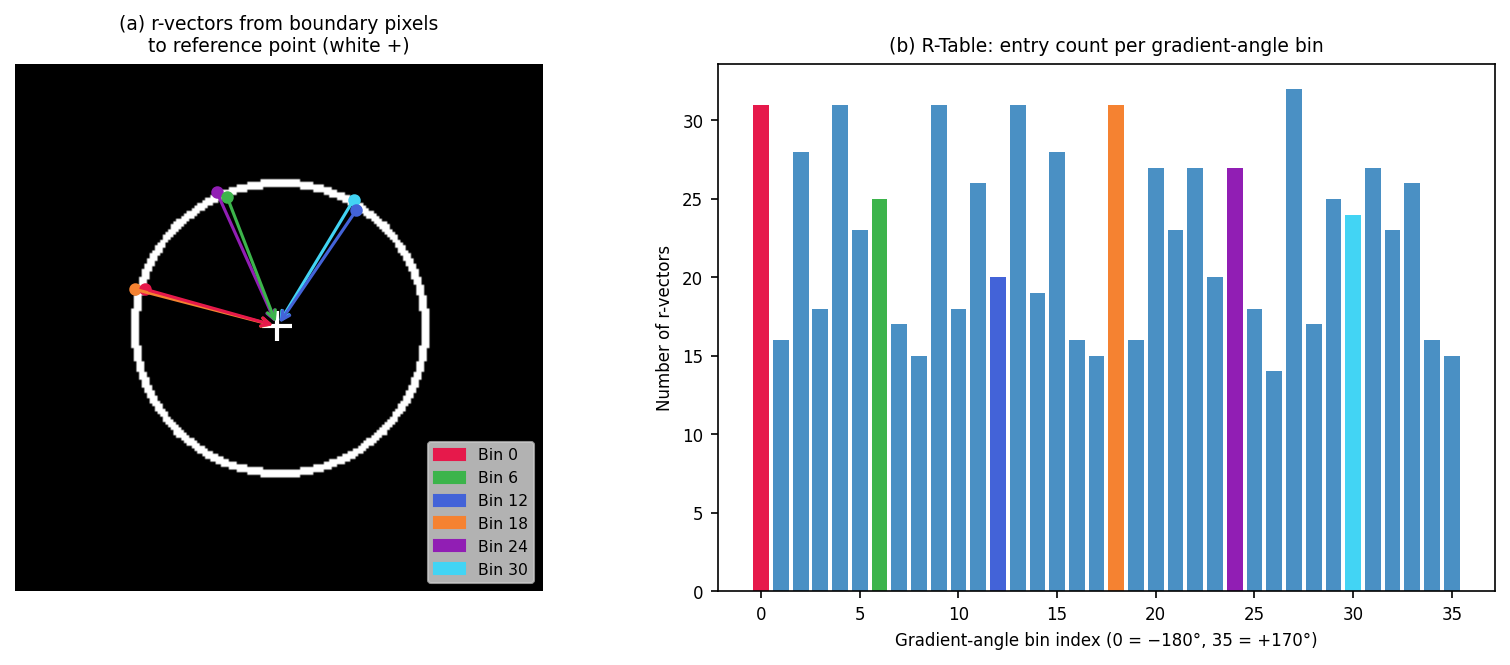
\includegraphics[width=0.85\textwidth]{figures/fig2_rtable.png}
  \caption{R-table construction on a circle template.
  (a)~Six sampled edge pixels with their displacement vectors pointing to the
  reference point; colour distinguishes gradient-angle bin.
  (b)~Histogram of R-table entry counts per bin---bins spanning angles perpendicular
  to the horizontal and vertical diameters hold the most entries.}
  \label{fig:rtable}
\end{figure}

\subsection{Detection Stage: Voting and Peak Finding}

\subsubsection*{Step 1 --- Preparing the Test Image}

Identical preprocessing such as Gaussian blur, Canny edge detection, Sobel gradient
estimation is run on the test image $I$ to produce its edge set $E'$ and
orientation map $\phi'$.  Using the same detector settings as during training ensures
that gradient angles are computed consistently between the two images.

\subsubsection*{Step 2 --- Accumulator Voting}

A zero-initialised array $A$ matching the dimensions of $I$ is the accumulator.
Each test edge pixel $(x, y)$ with bin $b$ looks up $R[b]$ and casts one vote for
every stored displacement vector:
\begin{equation}
  \forall\, (\Delta x, \Delta y) \in R[b]:\quad
  A[y + \Delta y]\,[x + \Delta x] \mathrel{+}= 1.
  \label{eq:voting}
\end{equation}
Whenever enough pixels agree on the same point, a
peak accumulates at that location.  Votes from unrelated image structures land at
inconsistent coordinates and remain scattered across $A$ without coalescing.

\begin{lstlisting}[caption={Accumulator voting: each edge pixel casts votes via its R-table bin.}]
H, W        = test_image.shape
accumulator = np.zeros((H, W), dtype=np.int32)

for x, y in zip(xs, ys):           # loop over test image edge pixels
    phi = angles[y, x]
    b   = int((phi + np.pi) / bin_width) % n_bins
    if b not in r_table:
        continue
    for rx, ry in r_table[b]:      # add displacement to get candidate ref location
        xv, yv = x + rx, y + ry
        if 0 <= xv < W and 0 <= yv < H:
            accumulator[yv, xv] += 1
\end{lstlisting}

\subsubsection*{Step 3 --- Locating the Peak}

Gradient quantisation means that nearby accumulator cells may each receive a few
votes that actually belong to the same peak.  A Gaussian smoothing pass with
kernel width $\sigma$ merges these before peak detection.  Candidate detections are
then identified as local maxima whose smoothed vote count clears a fraction $\tau$ of
the global maximum:
\begin{equation}
  \text{Detected} = \bigl\{(x,y) : A_\sigma(x,y) \geq \tau \cdot \max A_\sigma
  \;\text{and}\; A_\sigma \text{ is locally maximal}\bigr\},
\end{equation}
where $A_\sigma$ denotes the smoothed accumulator.  When more than one instance of
the shape is present, additional peaks are extracted through non-maximum suppression.

\begin{lstlisting}[caption={Gaussian smoothing followed by local-maximum peak detection.}]
smoothed  = cv2.GaussianBlur(accumulator.astype(np.float32), (0, 0), sigma)
local_max = (maximum_filter(smoothed, size=15) == smoothed)
peaks_msk = local_max & (smoothed >= threshold_ratio * smoothed.max())
ys, xs    = np.where(peaks_msk)   # coordinates of all surviving peaks
\end{lstlisting}

Figure~\ref{fig:voting} shows the three stages of the voting mechanism on a small
synthetic circle, making the convergence of votes toward the reference point visually
apparent.

\begin{figure}[H]
  \centering
  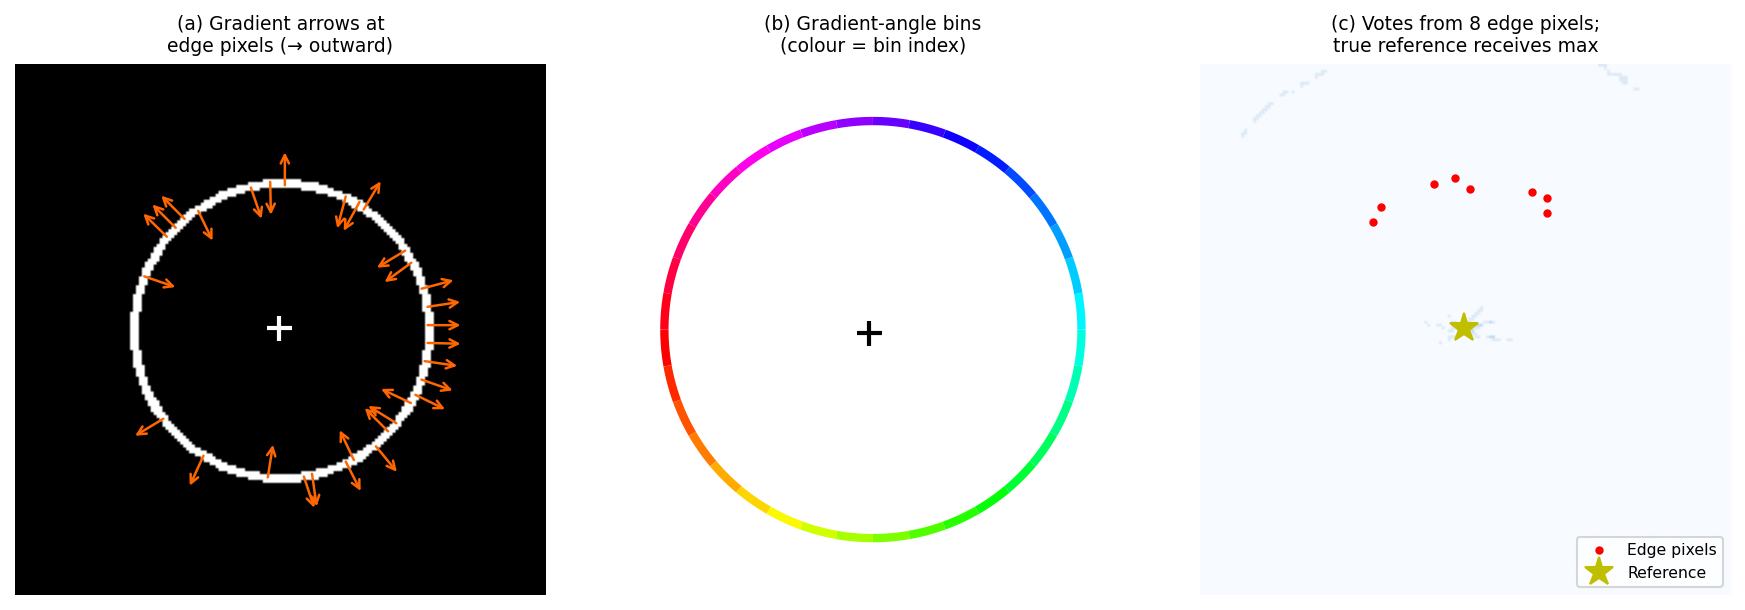
\includegraphics[width=0.90\textwidth]{figures/fig6_voting.png}
  \caption{Voting mechanism illustrated on a synthetic circle.
  (a)~Outward gradient arrows at a subset of edge pixels.
  (b)~Gradient-angle bins colour-coded around the boundary.
  (c)~Votes contributed by 8 sampled edge pixels. The true reference point
  accumulates the highest concentration.}
  \label{fig:voting}
\end{figure}

% ═════════════════════════════════════════════════════════════════════════════
\section{Pseudocode}
\label{sec:pseudocode}
% ═════════════════════════════════════════════════════════════════════════════

The two-phase algorithm is stated formally below.  Algorithm~\ref{alg:train} encodes
the template into the R-table; Algorithm~\ref{alg:detect} uses that table to locate
the shape in a new image.

\begin{algorithm}[H]
\DontPrintSemicolon
\caption{GHT --- Training Phase}
\label{alg:train}
\KwIn{Template image $T$;\; reference point $(x_r, y_r)$;\; bin count $N$}
\KwOut{R-table $R$}
$E \leftarrow \textsc{CannyEdges}(T)$\;
$\phi \leftarrow \textsc{GradientOrientation}(T)$\;
Initialise $R[b] \leftarrow \emptyset$ for $b = 0, 1, \ldots, N{-}1$\;
\ForEach{edge pixel $(x_e, y_e) \in E$}{
  $b \leftarrow \bigl\lfloor (\phi(x_e, y_e) \bmod 2\pi) \;/\; (2\pi / N) \bigr\rfloor$\;
  Append displacement $(y_r - y_e,\; x_r - x_e)$ to $R[b]$\;
}
\Return{$R$}
\end{algorithm}

\vspace{1em}

\begin{algorithm}[H]
\DontPrintSemicolon
\caption{GHT --- Detection Phase}
\label{alg:detect}
\KwIn{Test image $I$;\; R-table $R$;\; bin count $N$}
\KwOut{Reference-point location(s) of detected shape instance(s)}
$E' \leftarrow \textsc{CannyEdges}(I)$\;
$\phi' \leftarrow \textsc{GradientOrientation}(I)$\;
Initialise $A[y][x] \leftarrow 0$ for all valid $(x, y)$\;
\ForEach{edge pixel $(x, y) \in E'$}{
  $b \leftarrow \bigl\lfloor (\phi'(x,y) \bmod 2\pi) \;/\; (2\pi / N) \bigr\rfloor$\;
  \ForEach{$(\Delta y, \Delta x) \in R[b]$}{
    $A[y + \Delta y][x + \Delta x] \mathrel{+}= 1$\;
  }
}
Smooth $A$ with a Gaussian kernel\;
\Return{coordinates of local maxima in $A$ above threshold $\tau$}
\end{algorithm}

% ═════════════════════════════════════════════════════════════════════════════
\section{Scale and Rotation Invariance}
\label{sec:scale_rotation}
% ═════════════════════════════════════════════════════════════════════════════

The formulation in Section~\ref{sec:algorithm} treats the template scale and
orientation as fixed.  In many practical scenarios the object to be detected may
appear at a different size or at an arbitrary angle.  Ballard~\cite{ballard1981}
addressed this by introducing a full parameter vector
$\mathbf{a} = (x_r, y_r, s, \theta)$, where $s$ is a scale factor and $\theta$ is
an in-plane rotation angle, and defining how the R-table must be transformed for each
$(s, \theta)$ pair before votes are cast.

\subsection{Handling Scale Changes}

If the test shape is scaled by factor $s$ relative to the template, every
displacement vector in the R-table needs to be stretched by the same factor before
it can point to the correct reference location:
\begin{equation}
  T_s[R(\phi)] = s \cdot R(\phi).
  \label{eq:scale_transform}
\end{equation}
In practice, rather than continuously stretching the table, a discrete set of scale
values $\{s_1, s_2, \ldots, s_{N_s}\}$ is swept.  For each $s_i$, a scaled R-table
is applied and votes accumulate in a 3-D array $A[y][x][s]$.  This is the
strategy used in Section~\ref{sec:results} for \texttt{Fig0941}: nine templates
spanning radii $18$--$50\,\text{px}$ cover the full range of dowel sizes visible in
the image.

\subsection{Handling Rotation Changes}

Rotating the test shape by angle $\theta$ shifts every gradient angle by the same
amount, so the bin lookup key is incorrect for every edge pixel.  Thus, we shift
the index into the R-table by $\theta$ and simultaneously rotate each stored
displacement vector:
\begin{equation}
  T_\theta[R(\phi)] = \text{Rot}\bigl[R((\phi - \theta) \bmod 2\pi),\; \theta\bigr].
  \label{eq:rotation_transform}
\end{equation}
As with scale, a discrete angular grid is swept and a 3-D accumulator
$A[y][x][\theta]$ is used.

\subsection{Computational Cost of the Extended Search}

Combining both extensions produces a 4-D accumulator $A[y][x][s][\theta]$, and the
time cost grows accordingly.  Table~\ref{tab:complexity} lists the complexity for
each configuration.  The experimental results in Section~\ref{sec:analysis} show
concretely how detection degrades when scale and rotation compensation are omitted.

\begin{table}[H]
\centering
\caption{Computational complexity for different invariance configurations.
$N_e$: edge pixel count; $K$: mean R-table entries per bin;
$N_\theta$: rotation steps; $N_s$: scale steps.}
\label{tab:complexity}
\renewcommand{\arraystretch}{1.3}
\begin{tabular}{@{} l c c @{}}
\toprule
\textbf{Configuration} & \textbf{Accumulator dim.} & \textbf{Time complexity} \\
\midrule
Translation only               & 2-D: $(x, y)$             & $O(N_e \cdot K)$ \\
Translation + rotation         & 3-D: $(x, y, \theta)$     & $O(N_e \cdot K \cdot N_\theta)$ \\
Translation + scale            & 3-D: $(x, y, s)$          & $O(N_e \cdot K \cdot N_s)$ \\
Translation + rotation + scale & 4-D: $(x, y, \theta, s)$  & $O(N_e \cdot K \cdot N_\theta \cdot N_s)$ \\
\bottomrule
\end{tabular}
\end{table}

% ═════════════════════════════════════════════════════════════════════════════
\section{Step-by-Step Worked Example}
\label{sec:worked}
% ═════════════════════════════════════════════════════════════════════════════

\subsection{FigP0917 (noisy\_rectangle)}

This section follows
every intermediate result produced by the GHT on \texttt{FigP0917}
(\textit{noisy\_rectangle}), a binary image measuring $1247 \times 1294$\,px whose
rectangular boundary has been deliberately corrupted with noise.

The image is downscaled by $0.4$ before processing, both to reduce computation time
and because the downsampling averages out some of the fine-grained boundary noise.
The same image is used as both template and test to confirm that the R-table is constructed correctly.  If the algorithm is working, the
detected reference point should coincide with the template reference point.

Figure~\ref{fig:noisy_rect_steps} shows all six intermediate results in sequence.
The reference centroid computed from the template edges is $(248, 256)$.  The
detected accumulator peak lands at exactly $(248, 256)$ where offset $(\Delta x, \Delta
y) = (0, 0)$ is, confirming correct detection despite the noisy boundary.

\begin{figure}[H]
  \centering
  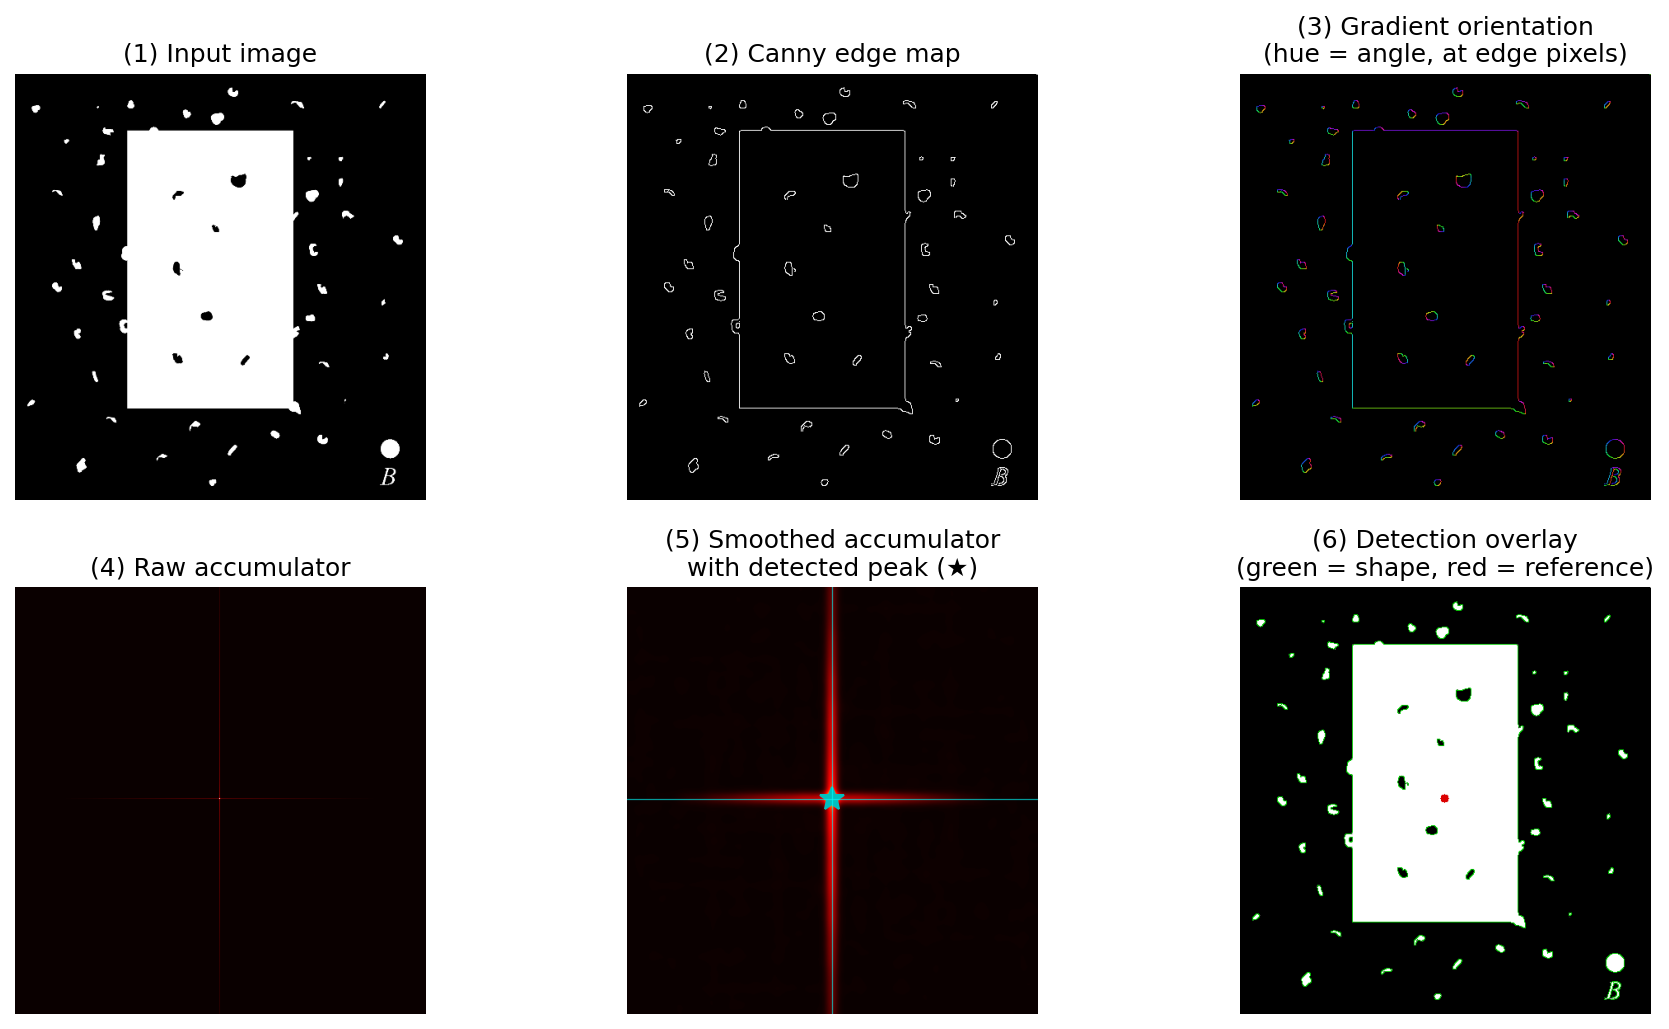
\includegraphics[width=\textwidth]{figures/fig3_noisy_rect_steps.png}
  \caption{Complete GHT execution trace on \texttt{FigP0917} (noisy rectangle).
  (1)~Downscaled input (2)~Canny edge map showing the jagged boundary
  (3)~gradient orientation visualised as hue at each edge pixel
  (4)~raw vote accumulator before smoothing;
  (5)~Gaussian-smoothed accumulator with the detected peak marked
  (6)~final detection. the green contour shows the projected template boundary
  and the red dot marks the recovered reference point.}
  \label{fig:noisy_rect_steps}
\end{figure}

Table~\ref{tab:rtable_sample} lists eight representative rows of the actual R-table
produced for this template.  The four straight sides of the rectangle dominate: bins
aligned with $-180^\circ$, $-90^\circ$, $0^\circ$, and $+90^\circ$ each collect
around 220--320 entries, reflecting the long runs of collinear edge pixels along each
side.  The diagonal bins collecting corner contributions hold far fewer vectors.
Every stored displacement has magnitude in the range 200--250\,px, consistent with
the distance from the boundary to the interior centroid.

\begin{table}[H]
\centering
\caption{Representative R-table entries for \texttt{FigP0917}.
Reference point $(248, 256)$; image downscaled $\times 0.4$; 72 bins of $5^\circ$
each.  Eight bins shown, spaced $45^\circ$ apart; three sample vectors per bin.}
\label{tab:rtable_sample}
\renewcommand{\arraystretch}{1.3}
\begin{tabular}{@{} c c r p{7cm} @{}}
\toprule
\textbf{Bin} & \textbf{Angle range} & \textbf{Entries} &
  \textbf{Sample $\mathbf{r} = (r_x, r_y)$} \\
\midrule
0  & $-180^\circ$ to $-175^\circ$ & 309 & $(-201,\;221)$,\; $(-102,\;215)$,\; $(-5,\;203)$ \\
9  & $-135^\circ$ to $-130^\circ$ &  47 & $(-21,\;229)$,\; $(147,\;214)$,\; $(-102,\;214)$ \\
18 & $-90^\circ$  to $-85^\circ$  & 237 & $(-250,\;255)$,\; $(-17,\;228)$,\; $(148,\;214)$ \\
27 & $-45^\circ$  to $-40^\circ$  &  51 & $(-249,\;255)$,\; $(-11,\;230)$,\; $(-93,\;219)$ \\
36 & $0^\circ$    to $+5^\circ$   & 318 & $(-249,\;256)$,\; $(-10,\;234)$,\; $(149,\;215)$ \\
45 & $+45^\circ$  to $+50^\circ$  &  44 & $(110,\;223)$,\; $(-198,\;221)$,\; $(84,\;190)$ \\
54 & $+90^\circ$  to $+95^\circ$  & 218 & $(-91,\;223)$,\; $(-92,\;223)$,\; $(-93,\;223)$ \\
63 & $+135^\circ$ to $+140^\circ$ &  26 & $(-15,\;238)$,\; $(-16,\;234)$,\; $(76,\;189)$ \\
\bottomrule
\end{tabular}
\end{table}

% ═════════════════════════════════════════════════════════════════════════════
\section{Results on Real Images}
\label{sec:results}
% ═════════════════════════════════════════════════════════════════════════════

\subsection{Fig0941 (wood\_dowels) --- Multi-Scale Detection}

\texttt{Fig0941} ($675 \times 531$\,px) presents a dense arrangement of wooden dowel
cross-sections photographed from above. To detect all possible sizes, nine circular templates are built at radii $\{18, 22, 26, 30, 34, 38, 42, 46, 50\}$
px.  Each produces its own accumulator, which is divided by the template's edge-pixel
count before smoothing. This normalisation prevents larger templates from
outscoring smaller ones purely by contributing more raw votes.  Smoothing uses a
radius-adaptive $\sigma = \max(3, r/8)$.  All nine normalised accumulators are then
merged into a single array by taking the element-wise maximum:
\begin{equation}
  A_\text{combined}(x,y) = \max_{r \in \mathcal{R}}\; A_r(x,y).
\end{equation}
Peak locations in $A_\text{combined}$ are extracted, and for each peak the radius is
assigned as whichever per-scale accumulator is highest at that location.
Non-maximum suppression keeps peaks separated by at least $0.65\,(r_1 + r_2)$, a
criterion chosen to permit adjacent-but-distinct dowels while rejecting duplicates:
the final tally is \textbf{48 detected dowels}.

\begin{figure}[H]
  \centering
  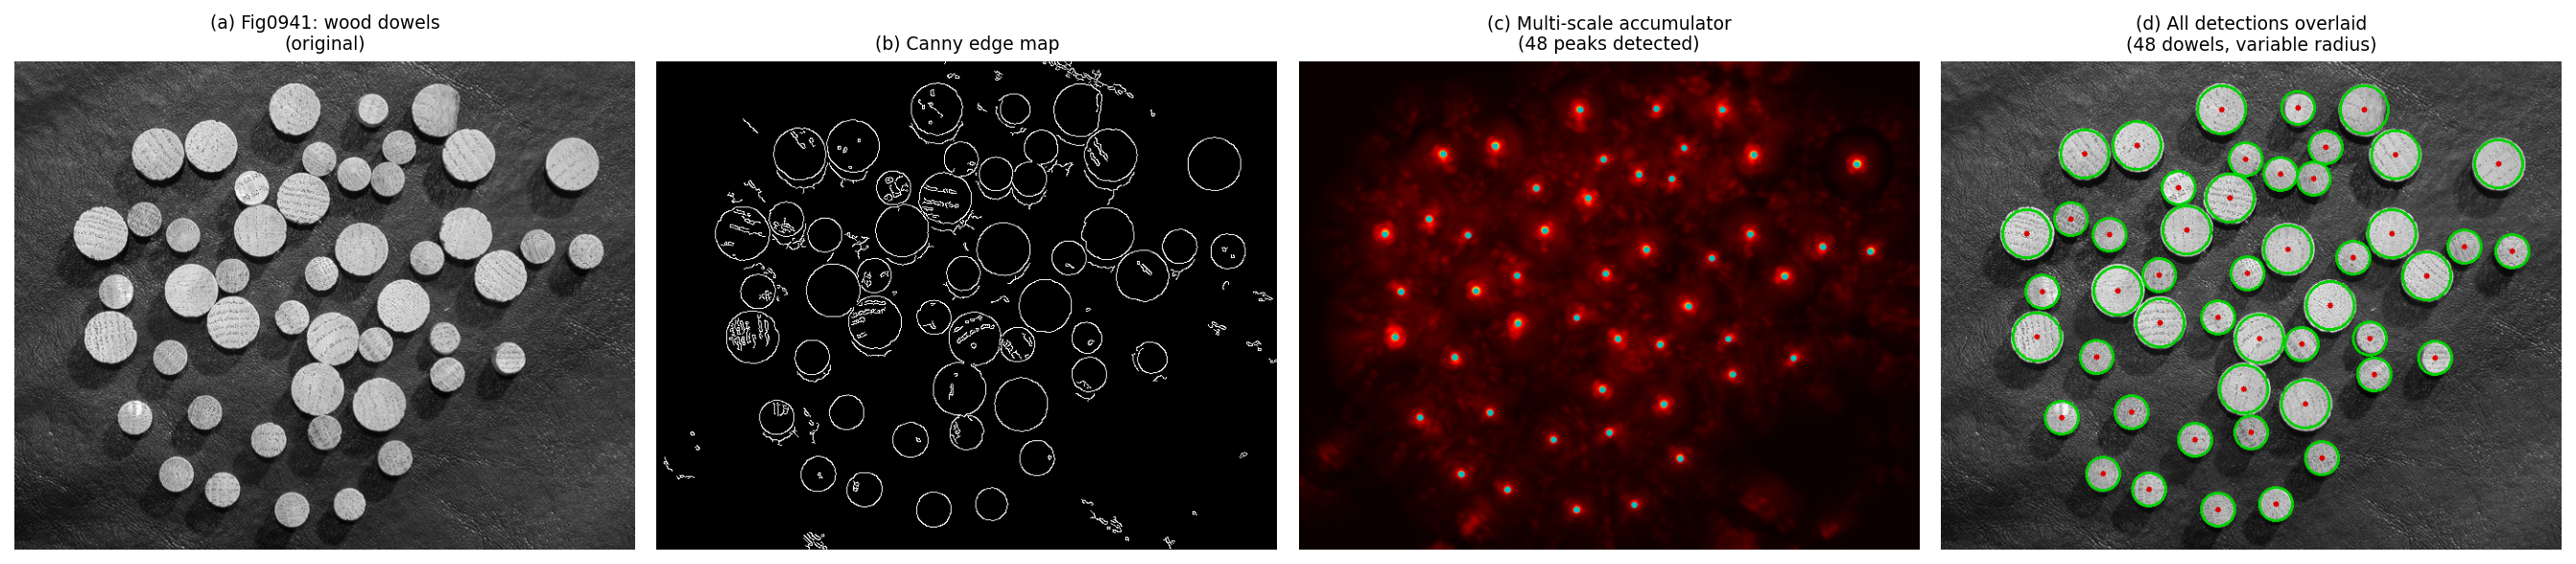
\includegraphics[width=\textwidth]{figures/fig4_dowels.png}
  \caption{Multi-scale GHT applied to \texttt{Fig0941} (wood dowels).
  (a)~Original image (b)~Canny edge map
  (c)~combined scale-max accumulator with the 48 detected peaks marked in cyan
  (d)~all 48 detections drawn on the original image with green circles sized
  to the individually estimated radius and red dots at each centre.}
  \label{fig:dowels}
\end{figure}

\begin{table}[H]
\centering
\caption{Parameters and results for \texttt{Fig0941} multi-scale GHT.}
\label{tab:dowels}
\renewcommand{\arraystretch}{1.3}
\begin{tabular}{@{} l l p{6.5cm} @{}}
\toprule
\textbf{Metric} & \textbf{Value} & \textbf{Notes} \\
\midrule
Radius range            & 18--50 px           & 9 templates, step size 4 px \\
Dowels detected         & 48                  & After radius-aware NMS \\
Accumulator threshold   & 28\% of max         & Threshold applied to combined array \\
NMS criterion           & $d < 0.65(r_1+r_2)$ & Allows closely packed but separate dowels \\
Normalisation           & $\div$ edge count   & Prevents large templates dominating \\
\bottomrule
\end{tabular}
\end{table}

\subsection{Fig1036 (septagon) --- Irregular Polygon Detection}

\texttt{Fig1036} ($814 \times 651$\,px) shows a single white seven-sided polygon
with a non-convex inward notch on its right side. The same image again serves as both template and test.  The reference point is computed
as the edge-pixel centroid at $(419, 325)$.  The GHT is then run on the same image,
and the detected peak is checked against this known reference.

\begin{figure}[H]
  \centering
  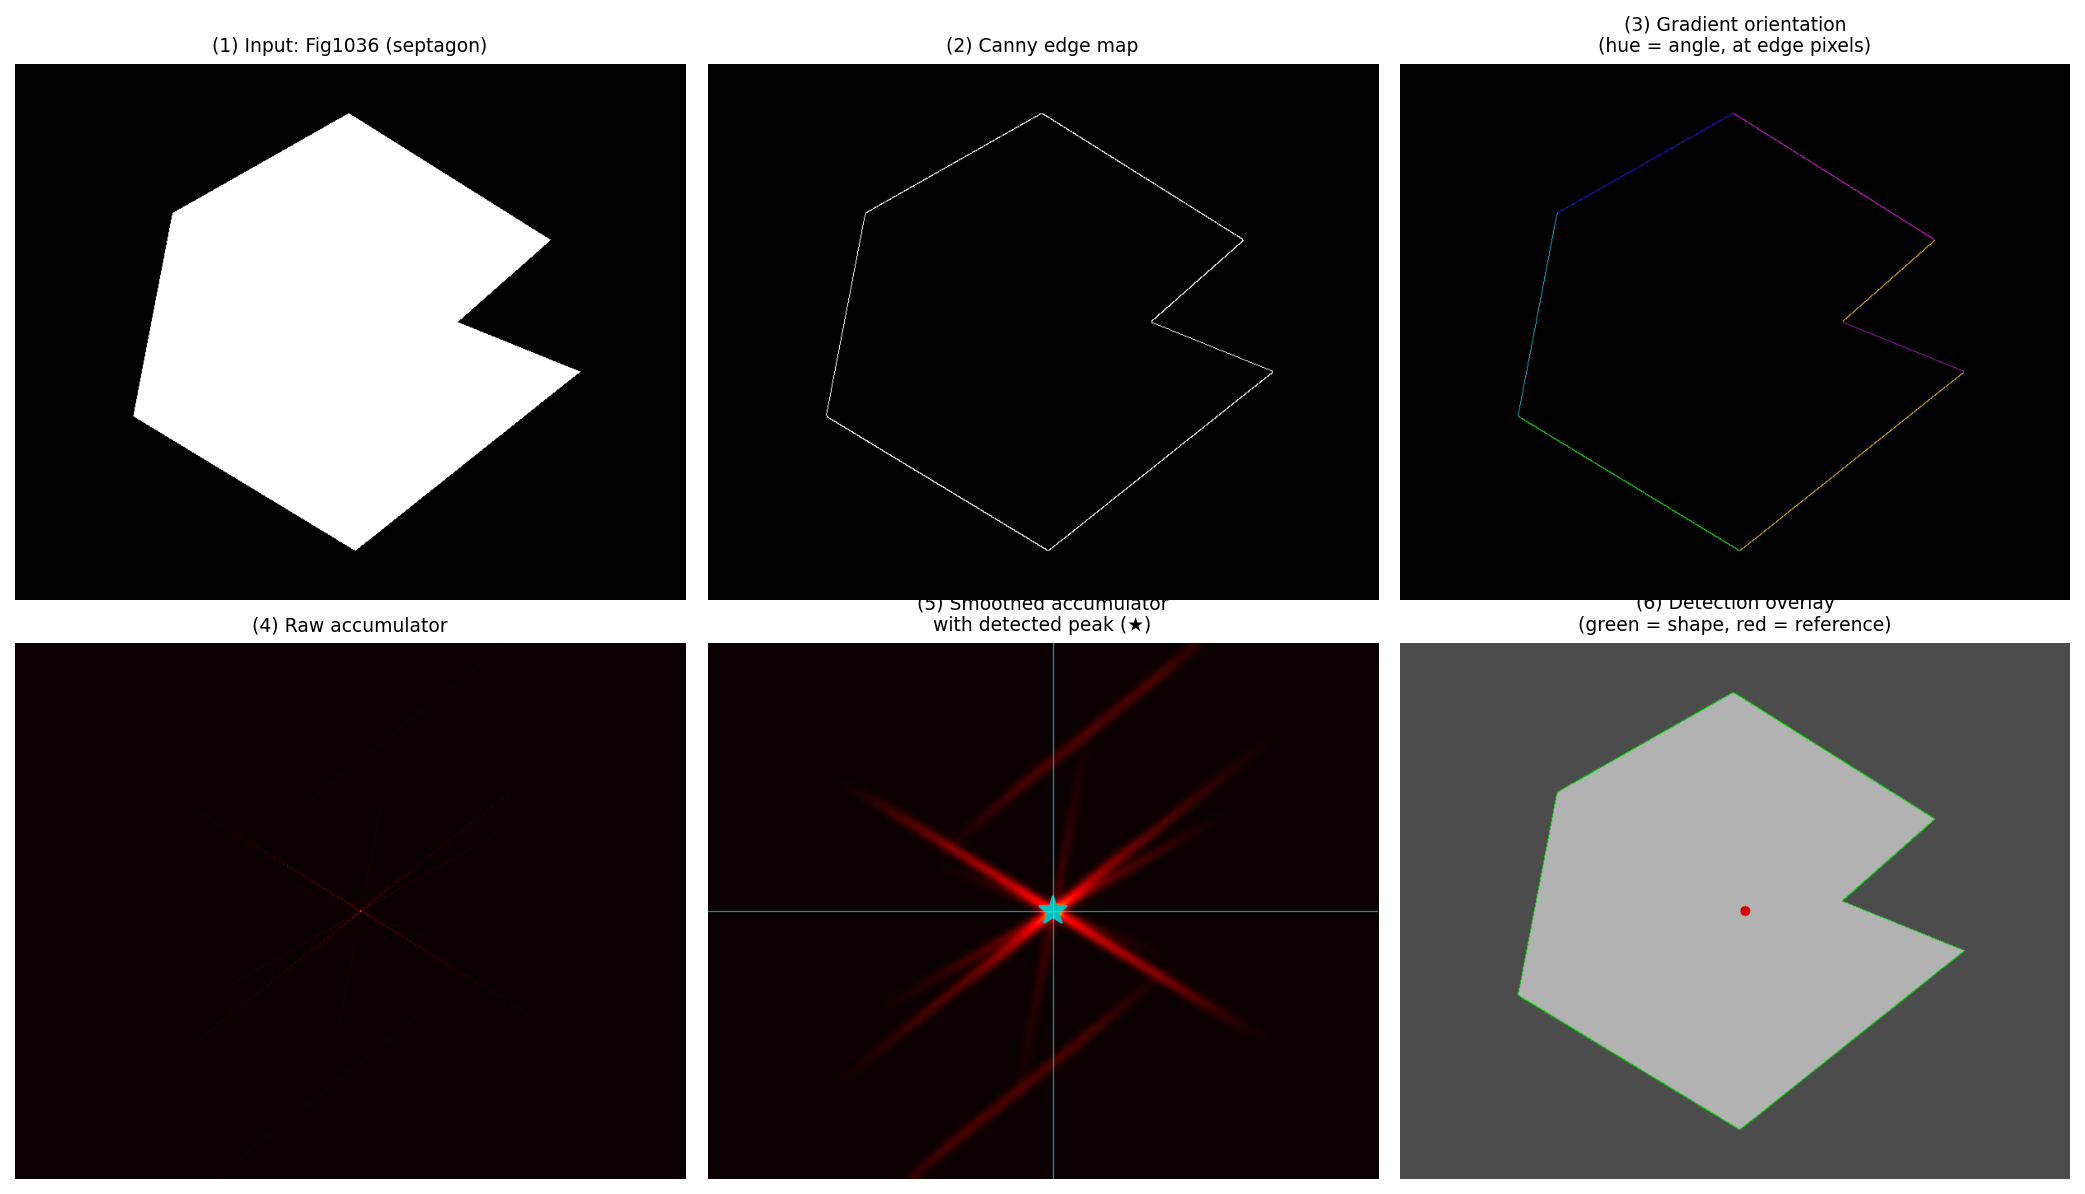
\includegraphics[width=\textwidth]{figures/fig_septagon_steps.png}
  \caption{Complete GHT trace on \texttt{Fig1036} (septagon).
  (1)~Input (2)~Canny edge map (3)~gradient orientation map
  (4)~raw accumulator (5)~smoothed accumulator with detected peak
  (6)~detection overlay with the green contour faithfully reproducing the full
  seven-sided boundary, including the non-convex notch.}
  \label{fig:septagon}
\end{figure}

In the raw accumulator in panel~(4) each straight side of
the polygon sends a concentrated line of votes toward the centroid, producing the
star-burst pattern visible there.  This pattern is distinctive to polygons and
contrasts sharply with the smooth circular halo seen for rounded shapes.  The
detected peak falls at $(419, 325)$ which is a perfect match to the template reference.  The overlay in panel~(6) traces the actual irregular
boundary, which no fixed parametric formula could have described.

\begin{table}[H]
\centering
\caption{Detection results for \texttt{Fig1036} (septagon).}
\label{tab:septagon}
\renewcommand{\arraystretch}{1.3}
\begin{tabular}{@{} l l p{6.5cm} @{}}
\toprule
\textbf{Metric} & \textbf{Value} & \textbf{Notes} \\
\midrule
Image dimensions      & $814 \times 651$\,px & Grayscale, uniform dark background \\
Template edge pixels  & 2113                 & Seven clean straight edges \\
Reference point       & $(419,\;325)$        & Centroid of boundary pixels \\
Detected peak         & $(419,\;325)$        & Zero positional error \\
Peak vote count       & 81                   & Sharp maximum; star-burst pattern \\
\bottomrule
\end{tabular}
\end{table}

\subsection{Fig0219 (rose) --- Robustness to Additive Noise}

\texttt{Fig0219} ($1024 \times 1024$\,px) is used here differently from the previous
two images: rather than testing whether a specific shape can be localised precisely,
it tests how well the voting mechanism tolerates additive pixel noise.  A circular
template of radius $180$\,px is used because the flower head is approximately
circular, but it is important to be clear that the detection overlay will show that
template circle, NOT a traced petal boundary, placed at the accumulator peak.

A $600 \times 600$ central crop of the image is processed twice: once clean and
once with zero-mean Gaussian noise of standard deviation $\sigma_n = 30$ added to
every pixel.  All algorithm parameters are held fixed between the two runs so that
the only variable is the noise level.

\begin{figure}[H]
  \centering
  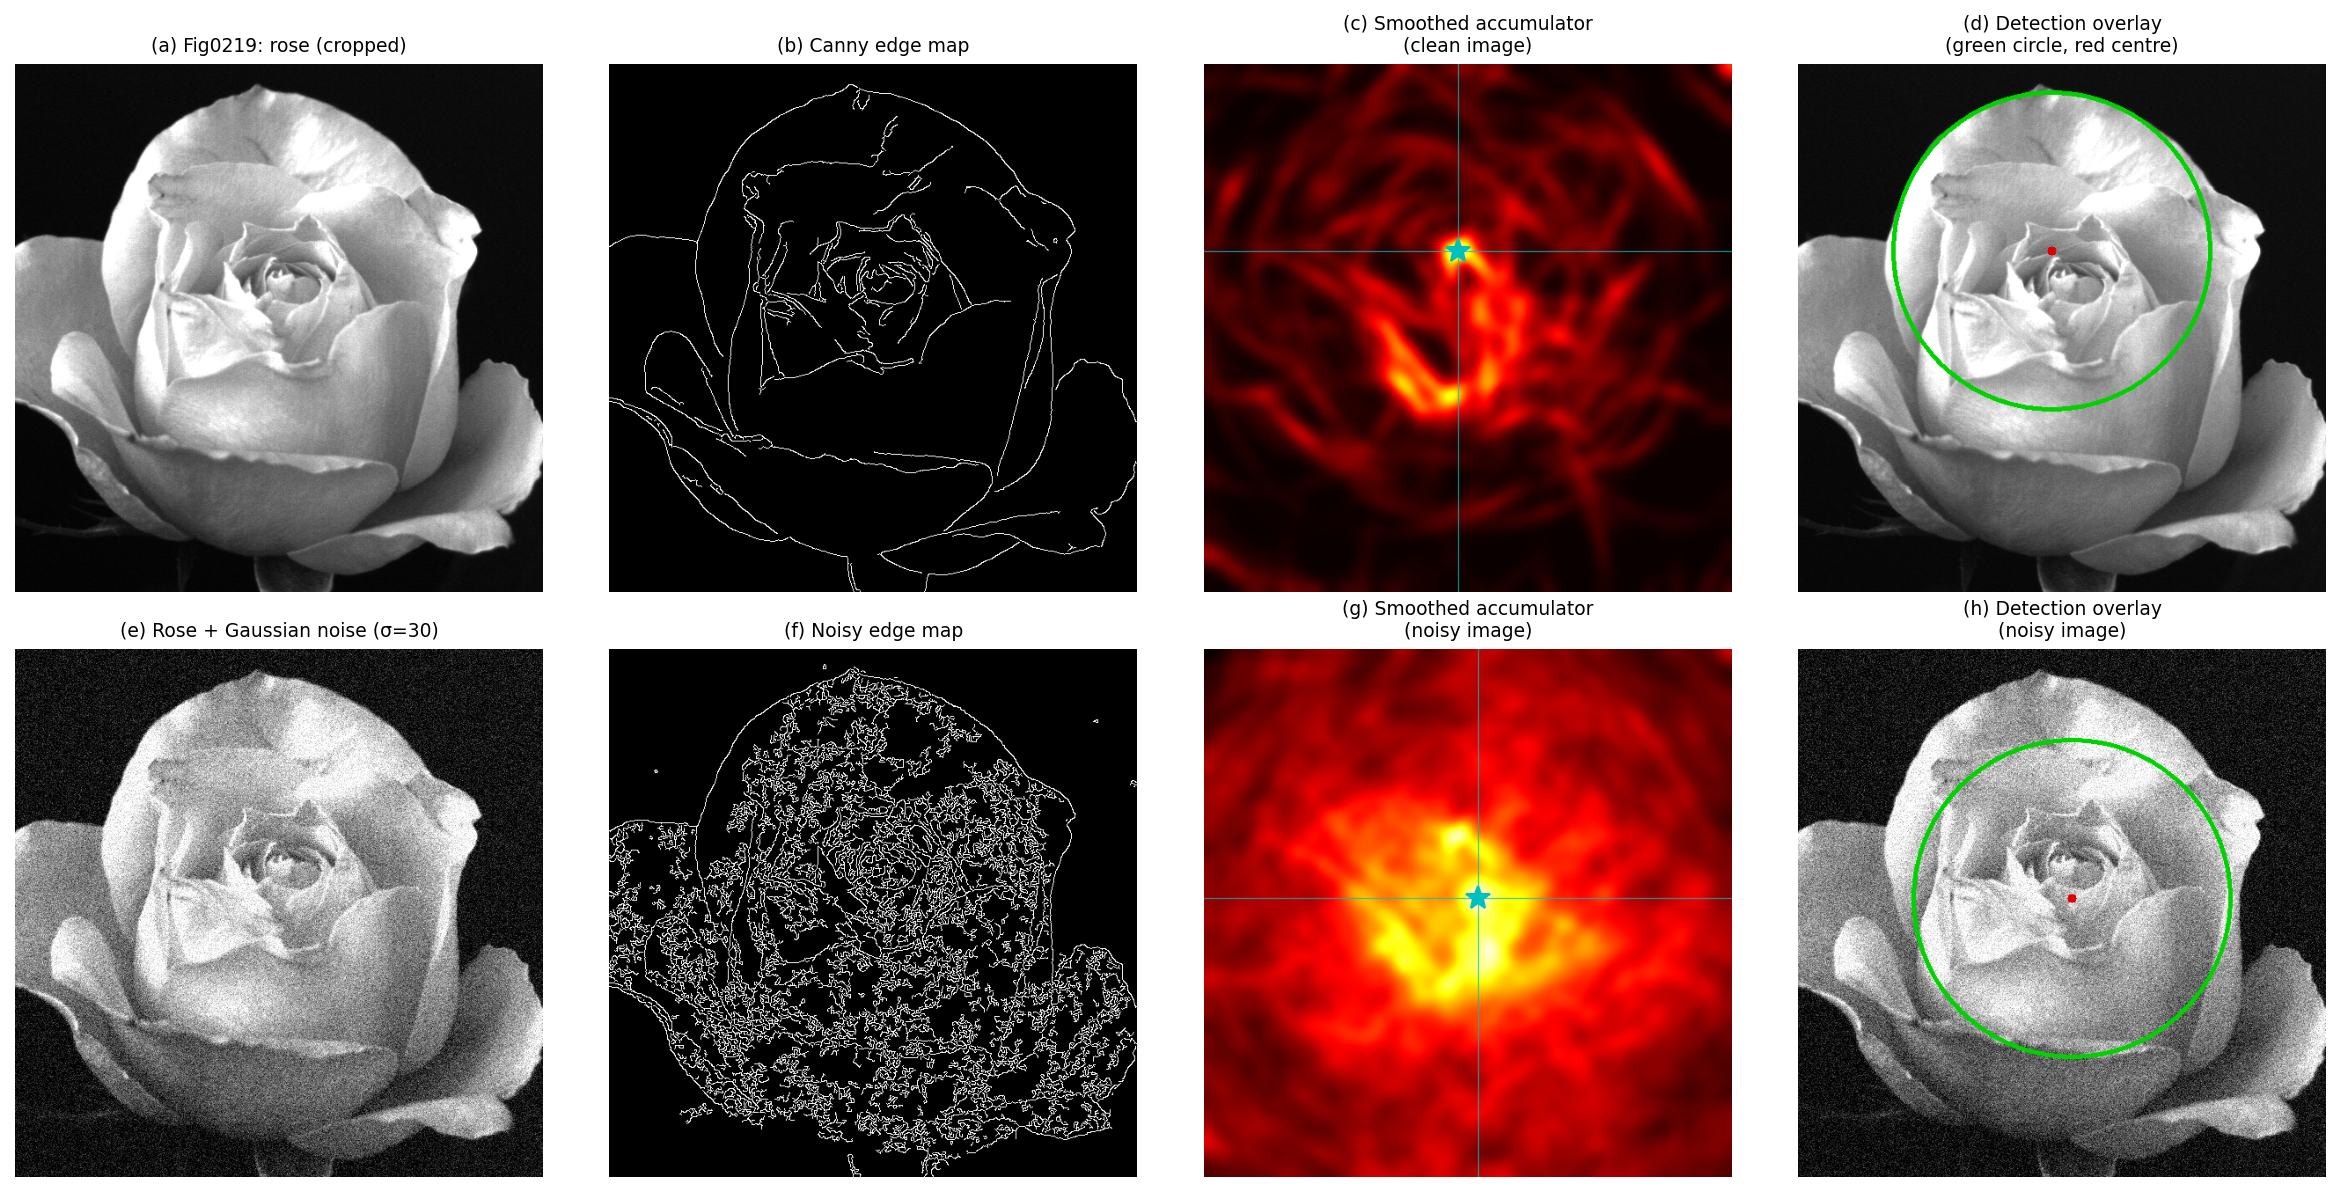
\includegraphics[width=\textwidth]{figures/fig5_rose.png}
  \caption{Noise robustness test on \texttt{Fig0219} (rose).
  Top row (clean input): (a)~cropped image (b)~Canny edges
  (c)~smoothed accumulator (d)~detected circular template overlaid.
  Bottom row (Gaussian noise $\sigma_n = 30$ added): (e)--(h) identical panels.
  The green boundary in (d) and (h) is the \emph{template circle}, not a
  traced petal outline.}
  \label{fig:rose}
\end{figure}

Comparing the two accumulator panels, the noisy version shows a markedly elevated
background as the large number of spurious Canny responses generated by noise each cast
a few votes at random locations, raising the floor across the entire array.  Despite
this, the flower-centre peak persists as the dominant maximum.  The votes contributed
by the genuine flower-boundary pixels are spatially coherent and converge, whereas
the noise-induced votes are random and therefore spread out.  As Illingworth and
Kittler~\cite{illingworth1988} note, this is a structural property of accumulator
voting: incoherent contributions cannot form a peak competitive with a coherent one
unless they vastly outnumber the true boundary pixels.

% ═════════════════════════════════════════════════════════════════════════════
\section{Experimental Analysis}
\label{sec:analysis}
% ═════════════════════════════════════════════════════════════════════════════

All experiments below use $N = 72$ gradient-angle bins and Gaussian smoothing
$\sigma = 5$ unless explicitly varied.  The three real images (\texttt{FigP0917},
\texttt{Fig1036}, \texttt{Fig0219}) serve as test subjects throughout.

\subsection{Robustness to Partial Occlusion}

A property of voting-based detection is that each boundary pixel
contributes its vote independently of every other pixel.  Blocking part of the shape
therefore removes some votes but leaves the remaining boundary pixels unaffected.
The net effect is that the accumulator peak shrinks in proportion to the occluded
fraction but does not disappear as long as enough boundary remains visible.

To measure this empirically, the right-hand portion of \texttt{FigP0917} is masked
to black in four increments: $0\%$, $25\%$, $50\%$, and $70\%$ of the image
width and the GHT is re-run each time using the unoccluded template R-table.

\begin{figure}[H]
  \centering
  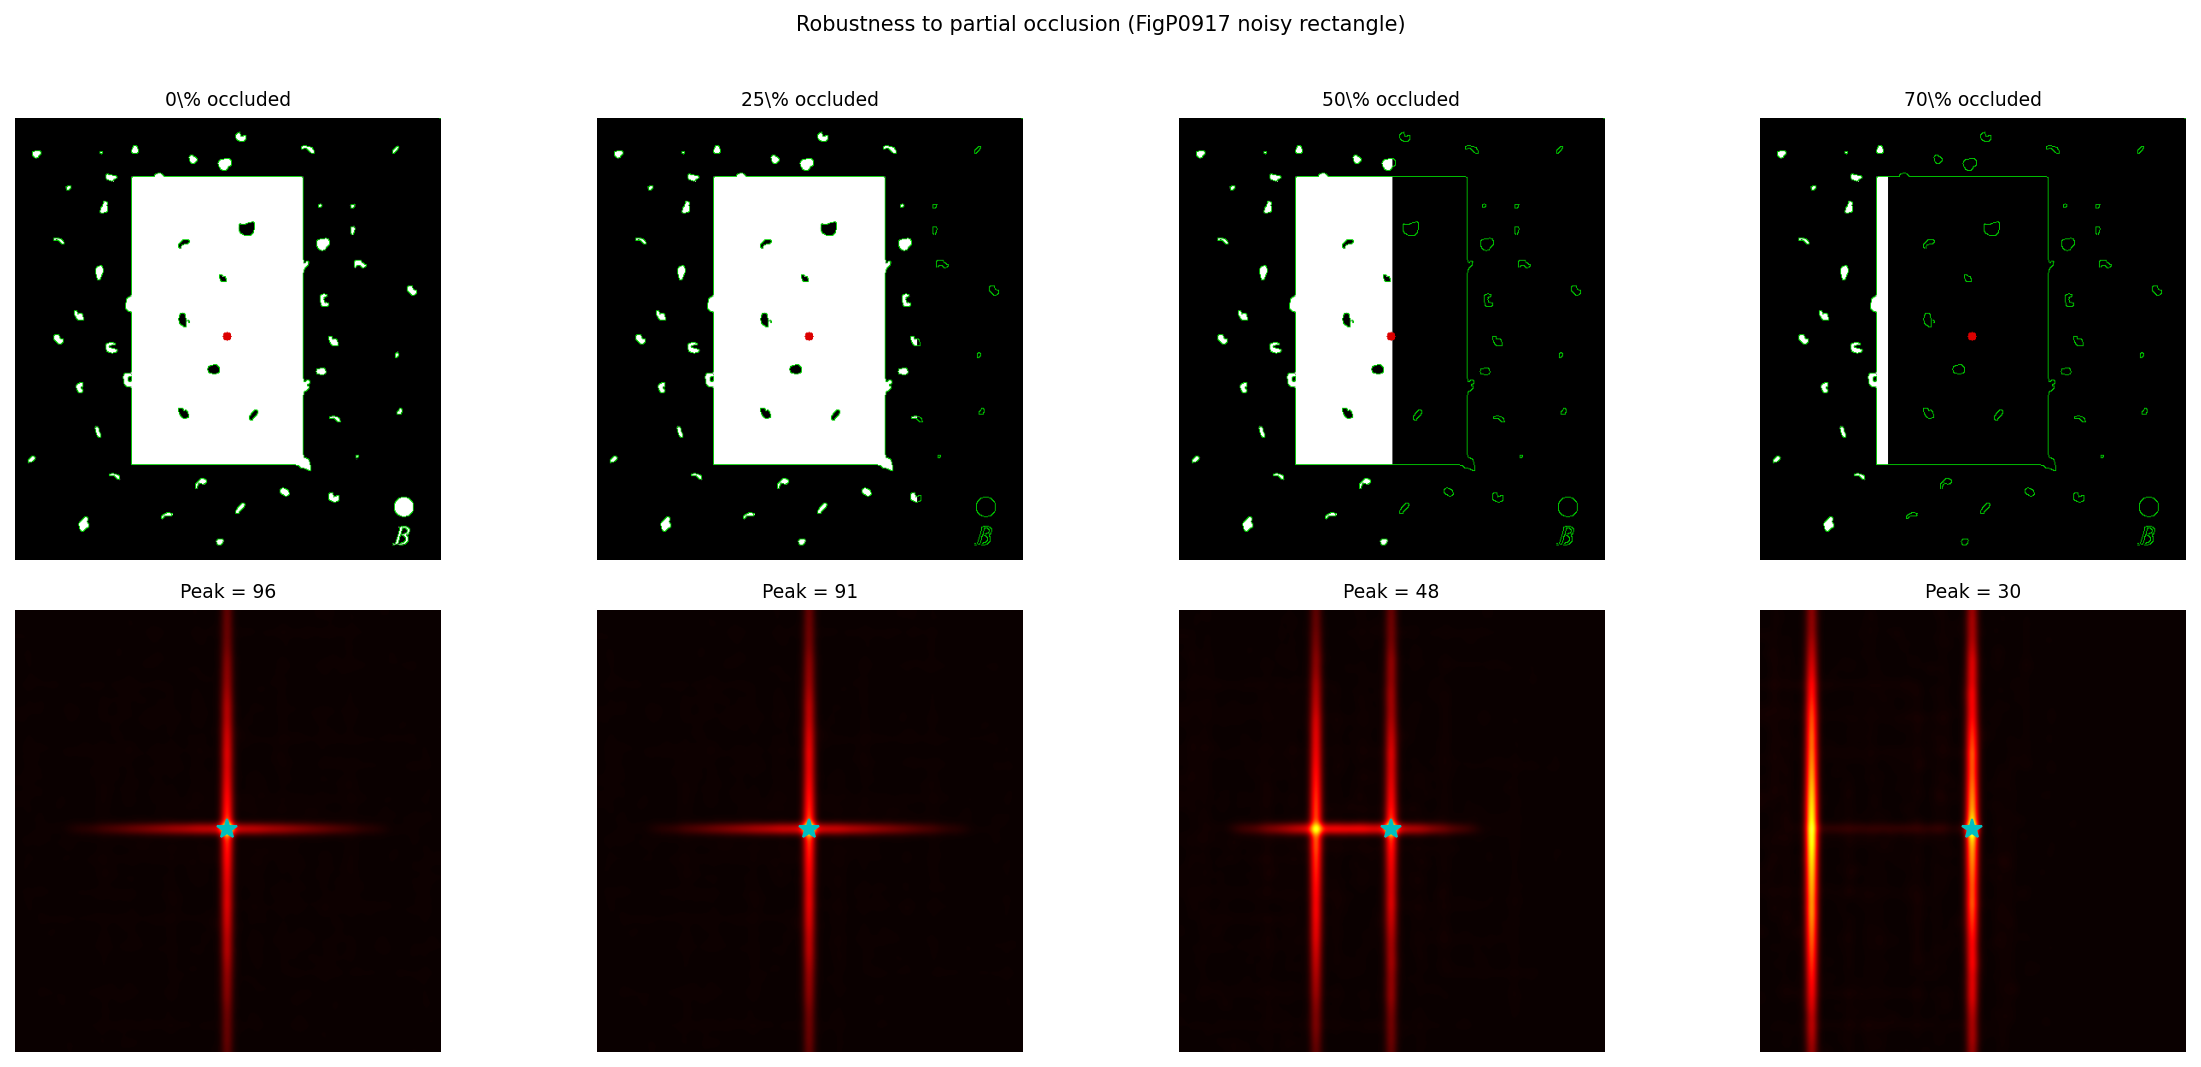
\includegraphics[width=\textwidth]{figures/fig_occlusion.png}
  \caption{Progressive occlusion applied to \texttt{FigP0917} (noisy rectangle).
  Top row: detection result at each occlusion level.
  Bottom row: smoothed accumulator with peak vote count annotated.
  The peak declines with the occluded fraction of boundary and collapses near 70\%.}
  \label{fig:occlusion}
\end{figure}

At $0\%$ the peak is the strongest and is well-localised.  At $25\%$ it is
noticeably weaker but the detection location is still correct.  By $50\%$ the
accumulator peak has roughly halved, consistent with losing approximately half the
contributing boundary pixels.  At $70\%$ the peak has fallen to the point where it
can no longer be reliably distinguished from the random accumulator floor generated
by the noisy boundary.  This proportional degradation is characteristic of
Hough-based methods~\cite{illingworth1988} and stands in contrast to feature-matching
approaches, which tend to fail more abruptly when key features are removed.

\subsection{Effect of Scale Mismatch}

When a fixed-scale R-table is applied to a test shape that appears at a different
size, the displacement vectors stored in the table no longer point to the correct
reference location.  Instead of all converging at a single cell, they land at a
scattered cloud of cells around the true reference.  The accumulator peak collapses
from a sharp spike to a broad, low mound.

\texttt{FigP0917} is resized to four scales---$0.5\times$, $0.75\times$, $1.0\times$,
$1.5\times$---and each resized version is tested against an R-table trained
exclusively at $1.0\times$.

\begin{figure}[H]
  \centering
  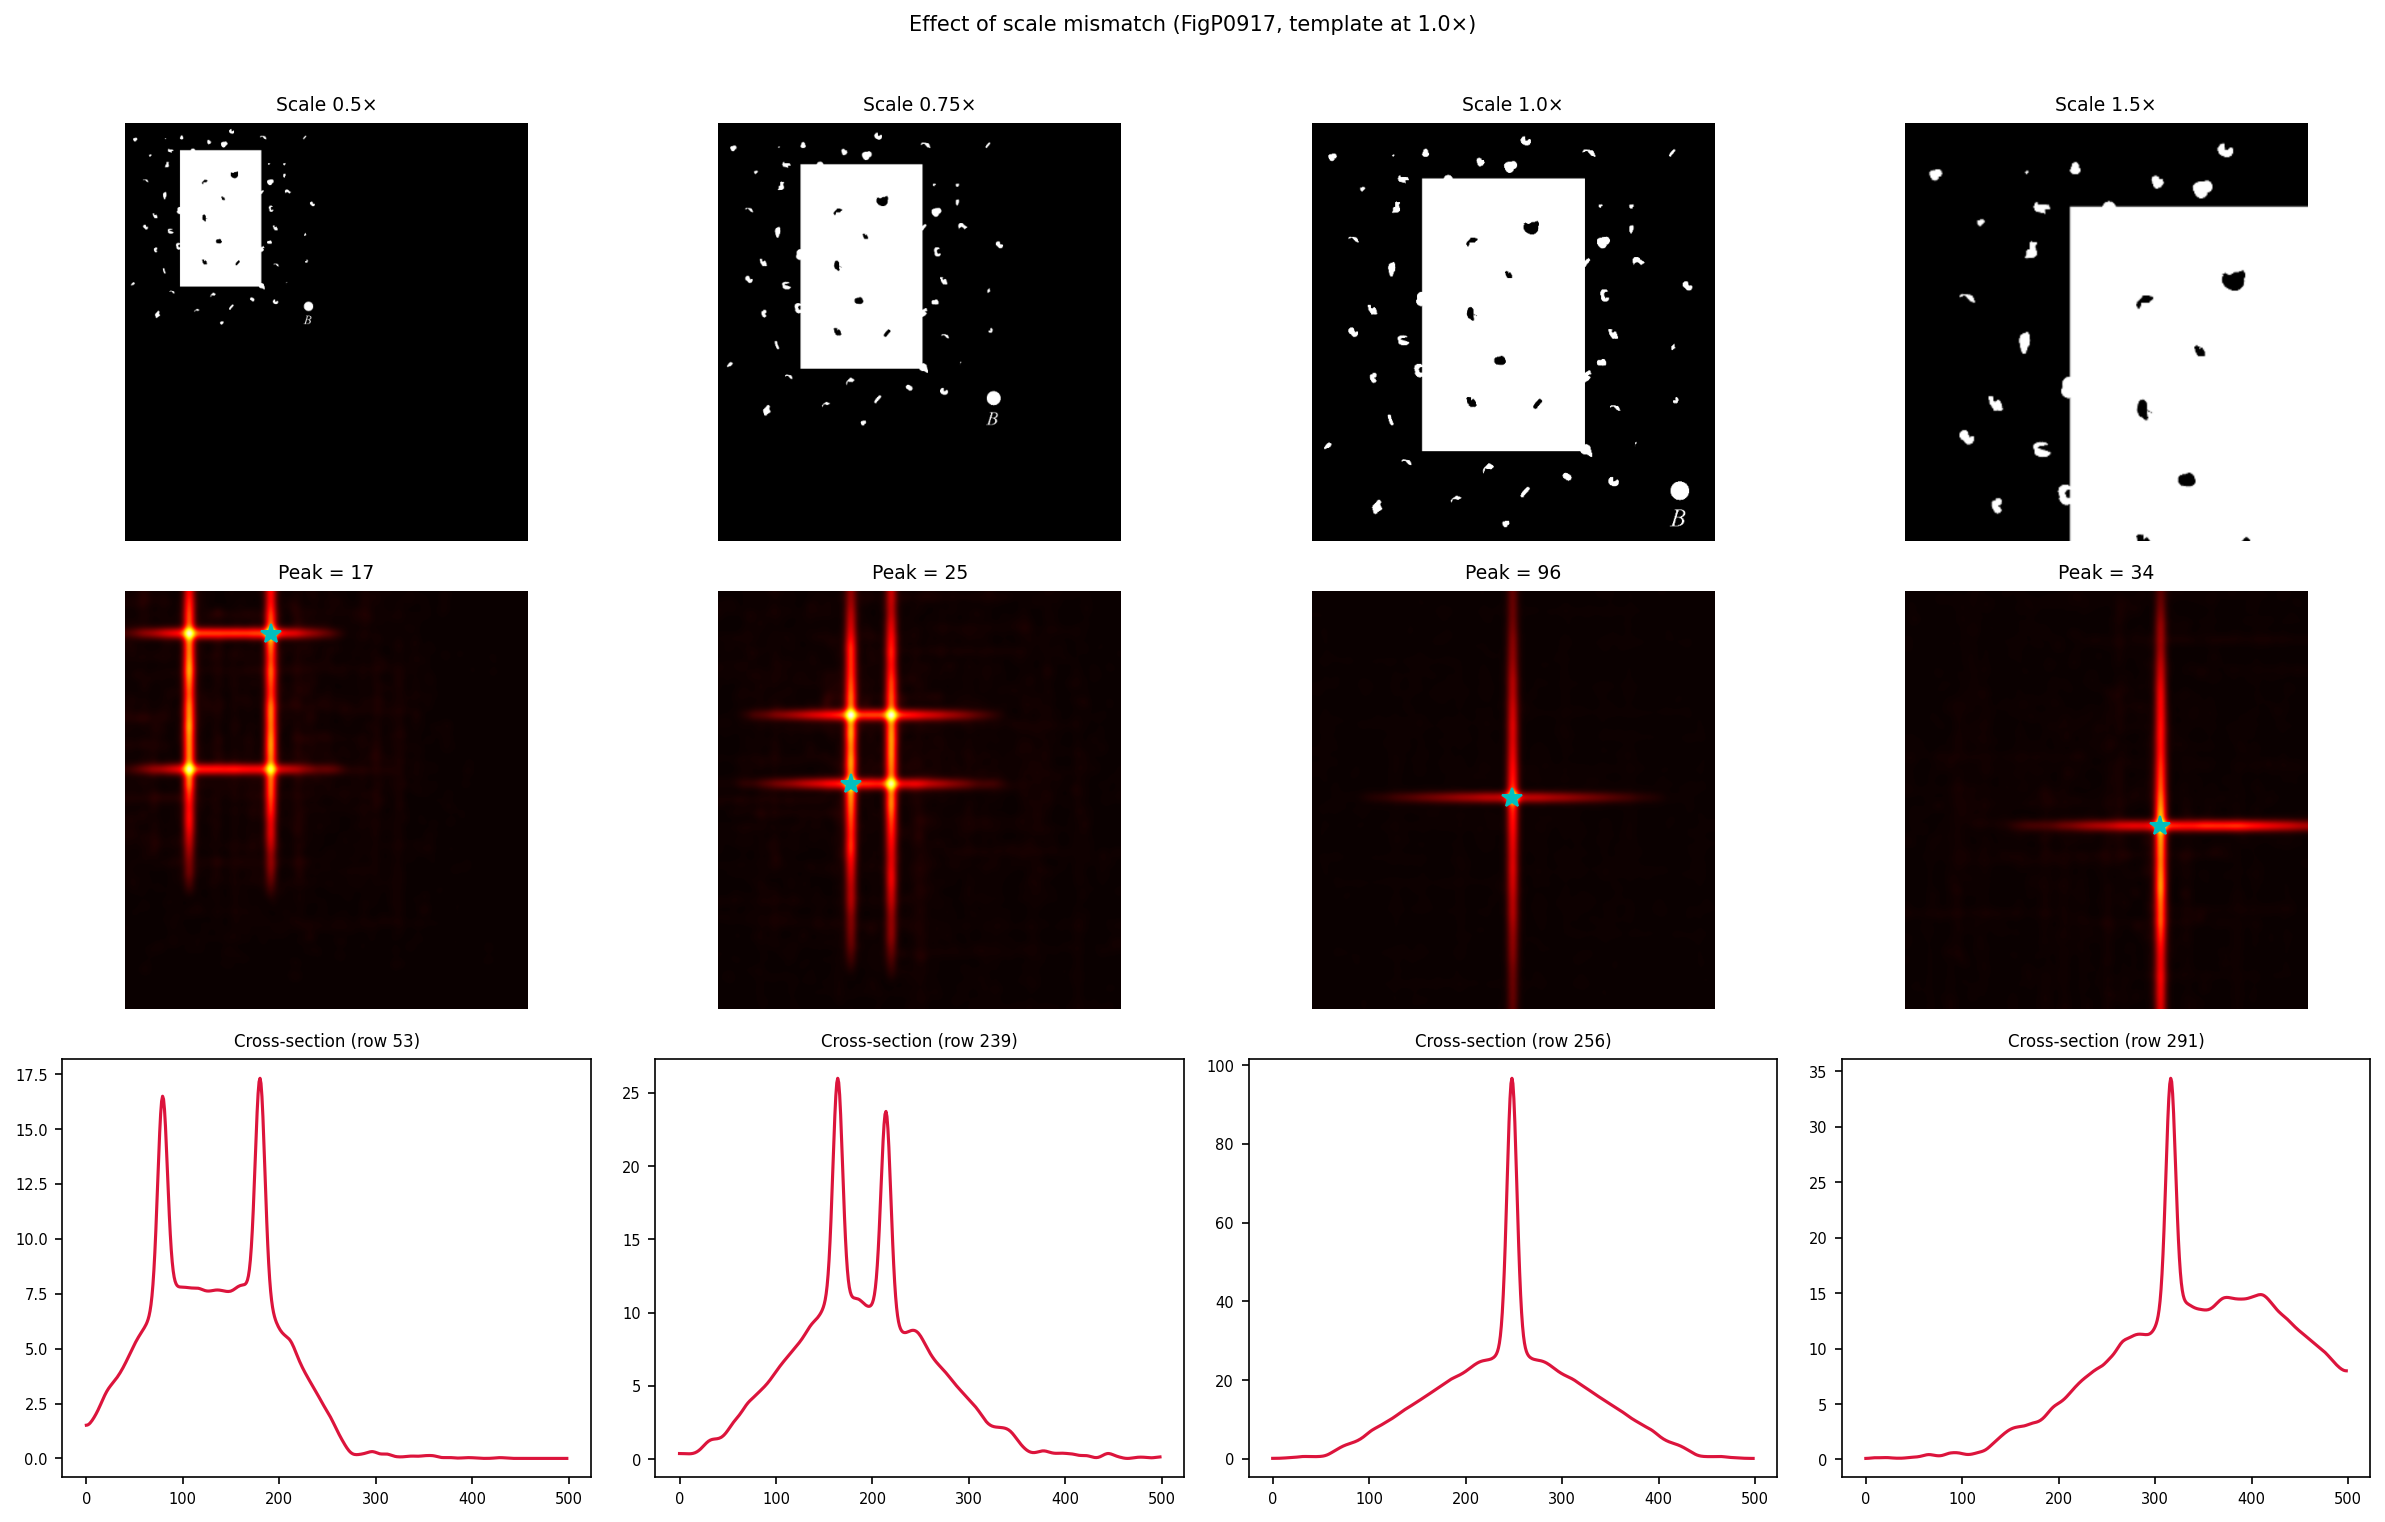
\includegraphics[width=\textwidth]{figures/fig_scale_mismatch.png}
  \caption{Scale mismatch test on \texttt{FigP0917} (template trained at $1.0\times$).
  Top: test images at each scale.  Middle: smoothed accumulators.
  Bottom: horizontal cross-sections through the peak row---only the matching
  scale produces a narrow spike.}
  \label{fig:scale_mismatch}
\end{figure}

From figure~\ref{fig:scale_mismatch} we can see that at $1.0\times$ the cross-section is a sharp spike with a high
amplitude.  At $0.5\times$ the test shape is half the size of the template, so
every stored displacement vector is twice as long as needed; the votes are smeared
outward from the true peak in a square-like pattern.  At $1.5\times$ the effect is
reversed as vectors are too short and votes cluster inside the true location.  In
both mismatched cases the peak amplitude drops dramatically.  This experiment
motivates the multi-scale approach applied to the wood dowels image, where nine
templates covering the full observed radius range are combined.

\subsection{Effect of Rotation Mismatch}

A rotation of the test shape shifts every gradient angle by the same offset $\theta$.
As a result, each test edge pixel looks up the wrong bin in the R-table, which is the
bin for orientation $\phi$ instead of orientation $\phi - \theta$, and retrieves
displacement vectors built for a different part of the boundary.  The votes scatter
rather than converge.

\texttt{Fig1036} (septagon) is rotated by $0^\circ$, $30^\circ$, $60^\circ$, and
$90^\circ$ and tested against the $0^\circ$ template.

\begin{figure}[H]
  \centering
  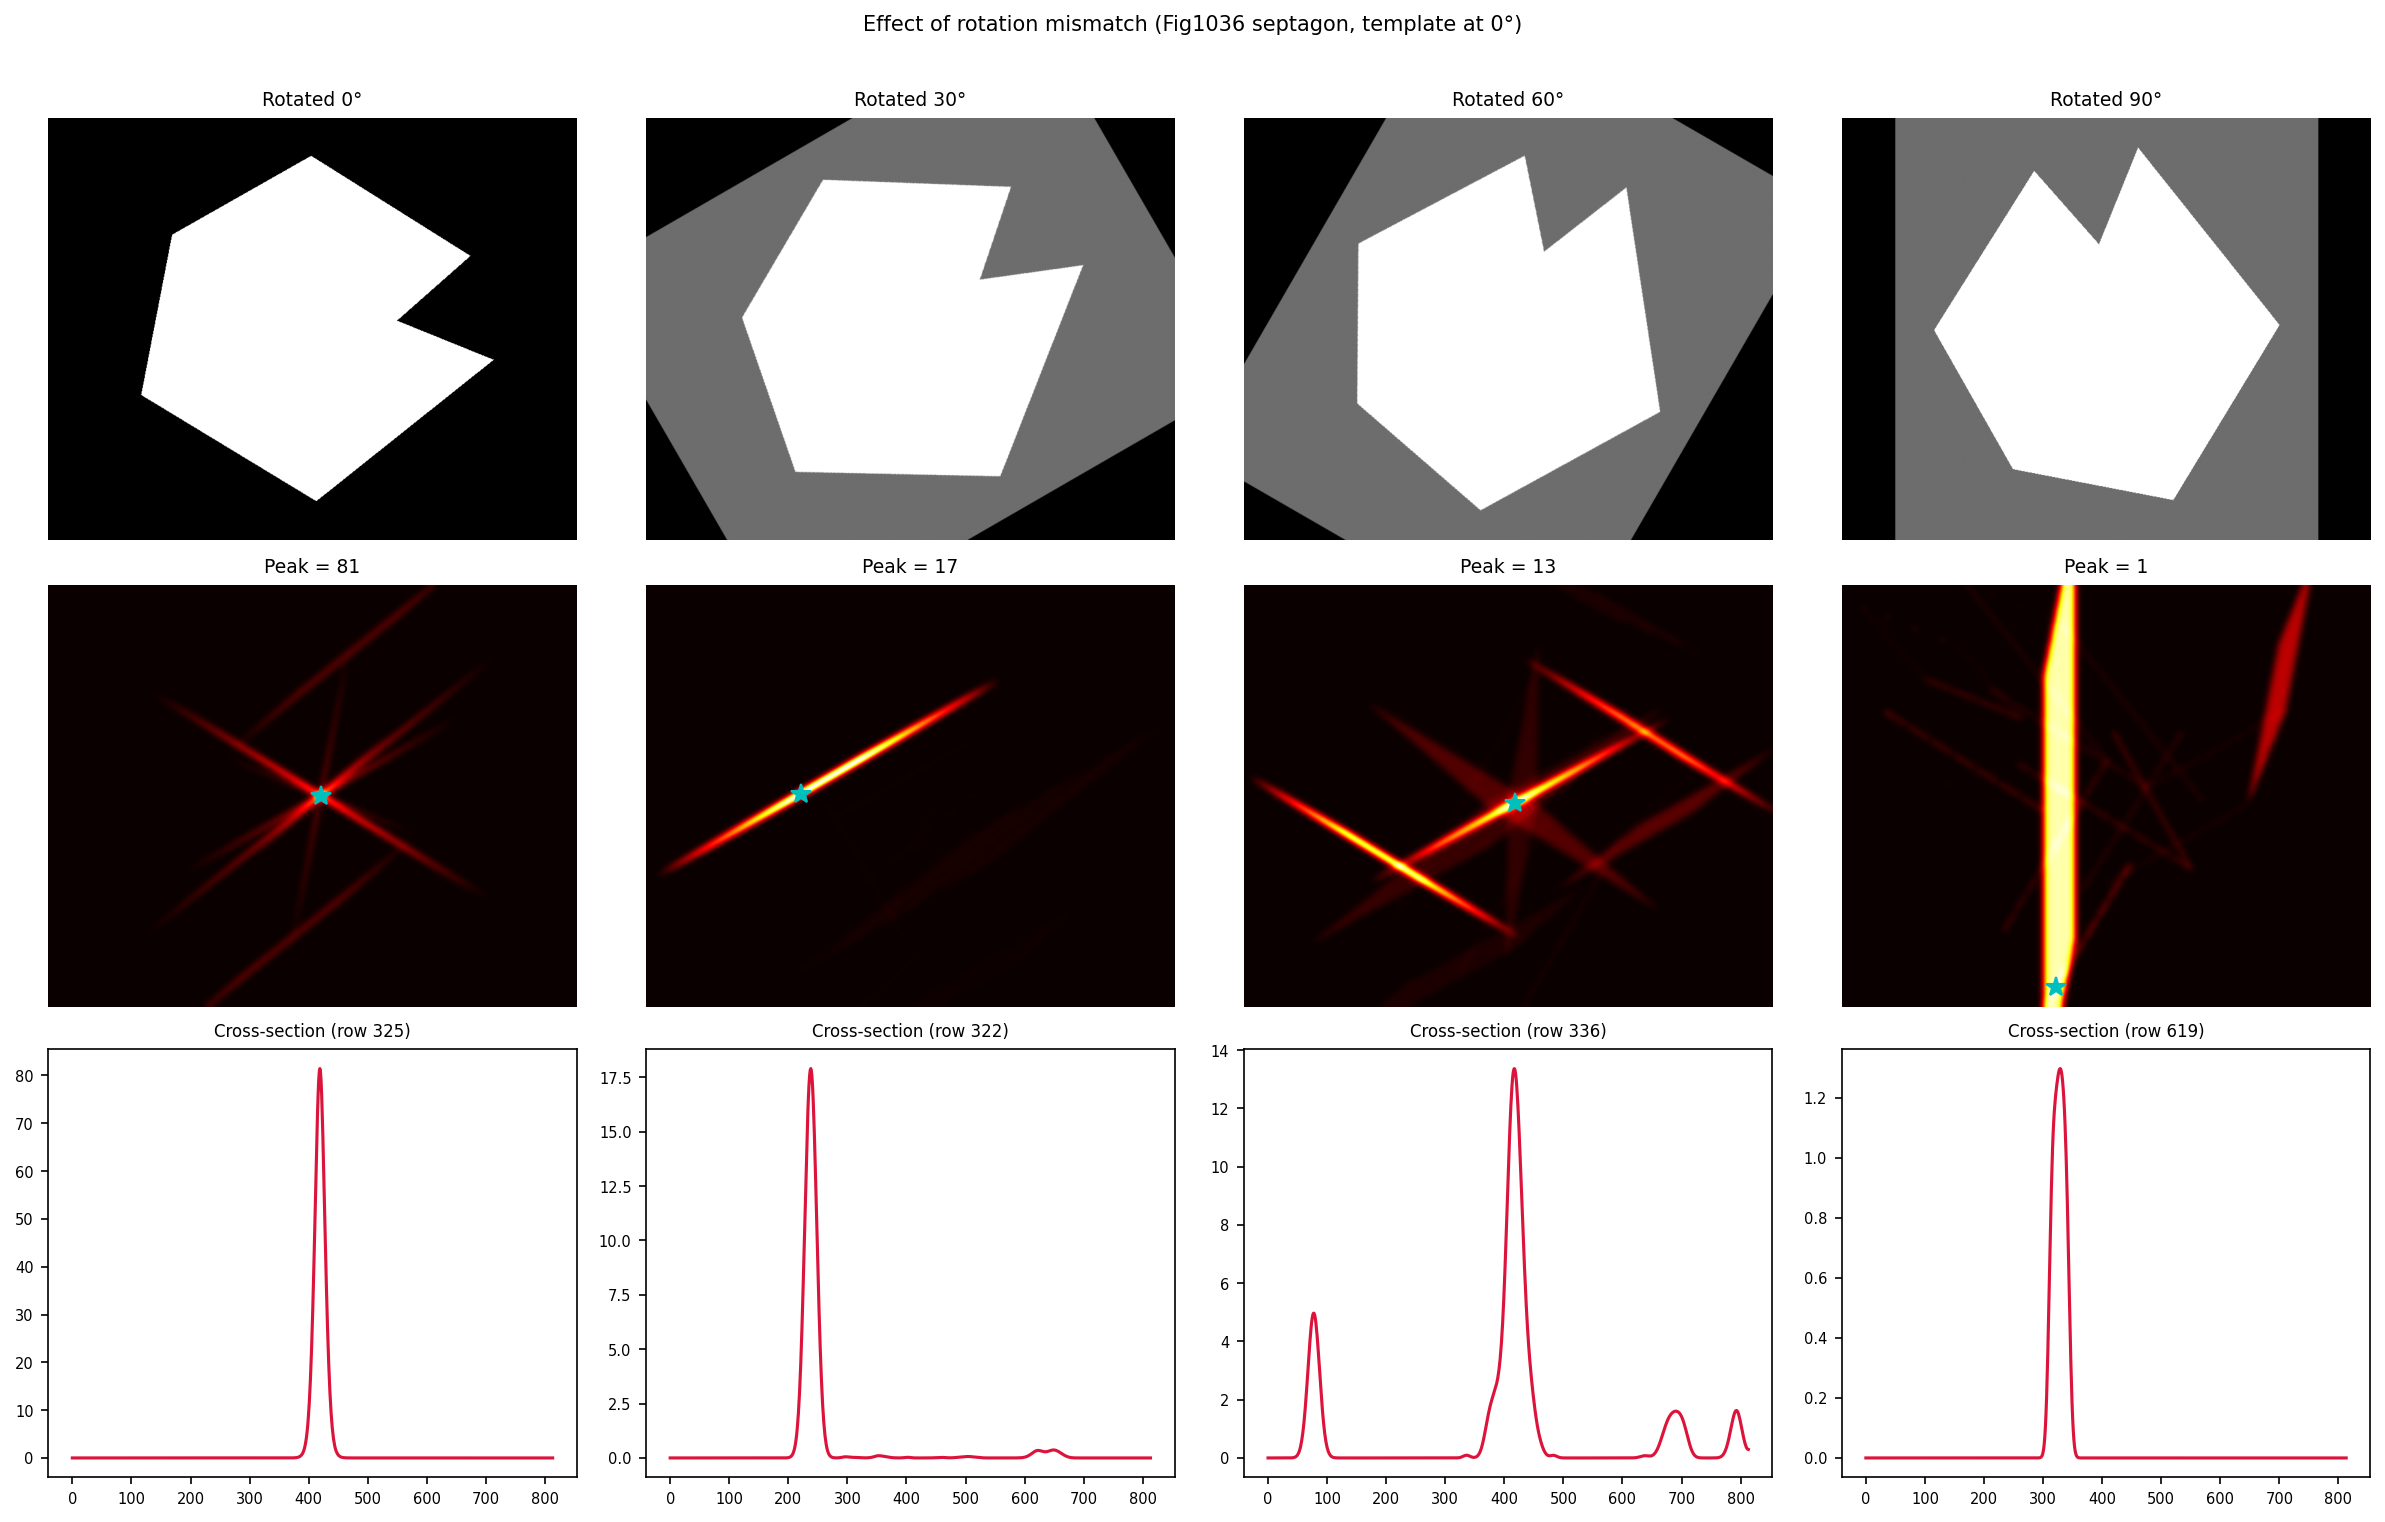
\includegraphics[width=\textwidth]{figures/fig_rotation_mismatch.png}
  \caption{Rotation mismatch test on \texttt{Fig1036} (septagon, template at $0^\circ$).
  Top: rotated test images.  Middle: smoothed accumulators.
  Bottom: horizontal cross-sections through the peak row.}
  \label{fig:rotation_mismatch}
\end{figure}

At $0^\circ$ the cross-section shows a clear spike above the background.  At
$30^\circ$ and $60^\circ$ the peak collapses to much lower votes because almost every gradient-angle lookup retrieves
the wrong displacement vectors.  At $90^\circ$ a slight partial recovery is possible
for shapes with approximate symmetry, but the septagon is asymmetric so the peak
remains negligible.  To handle arbitrary orientations the R-table would need to be
rotated according to Equation~\eqref{eq:rotation_transform} and a full angular sweep
performed, as outlined in Section~\ref{sec:scale_rotation}.

\subsection{Template Mismatch}

When the R-table is built from the wrong shape the displacement vectors associated with each gradient-angle bin
simply do not point toward any consistent location in the test image.  Votes are
deposited at a different spread of positions for every edge pixel, and the accumulator
fills up more or less uniformly without forming a peak.

Figure~\ref{fig:template_mismatch} applies three templates to the \texttt{Fig1036}
septagon: the correct septagon template, a circular template, and a rectangular
template.

\begin{figure}[H]
  \centering
  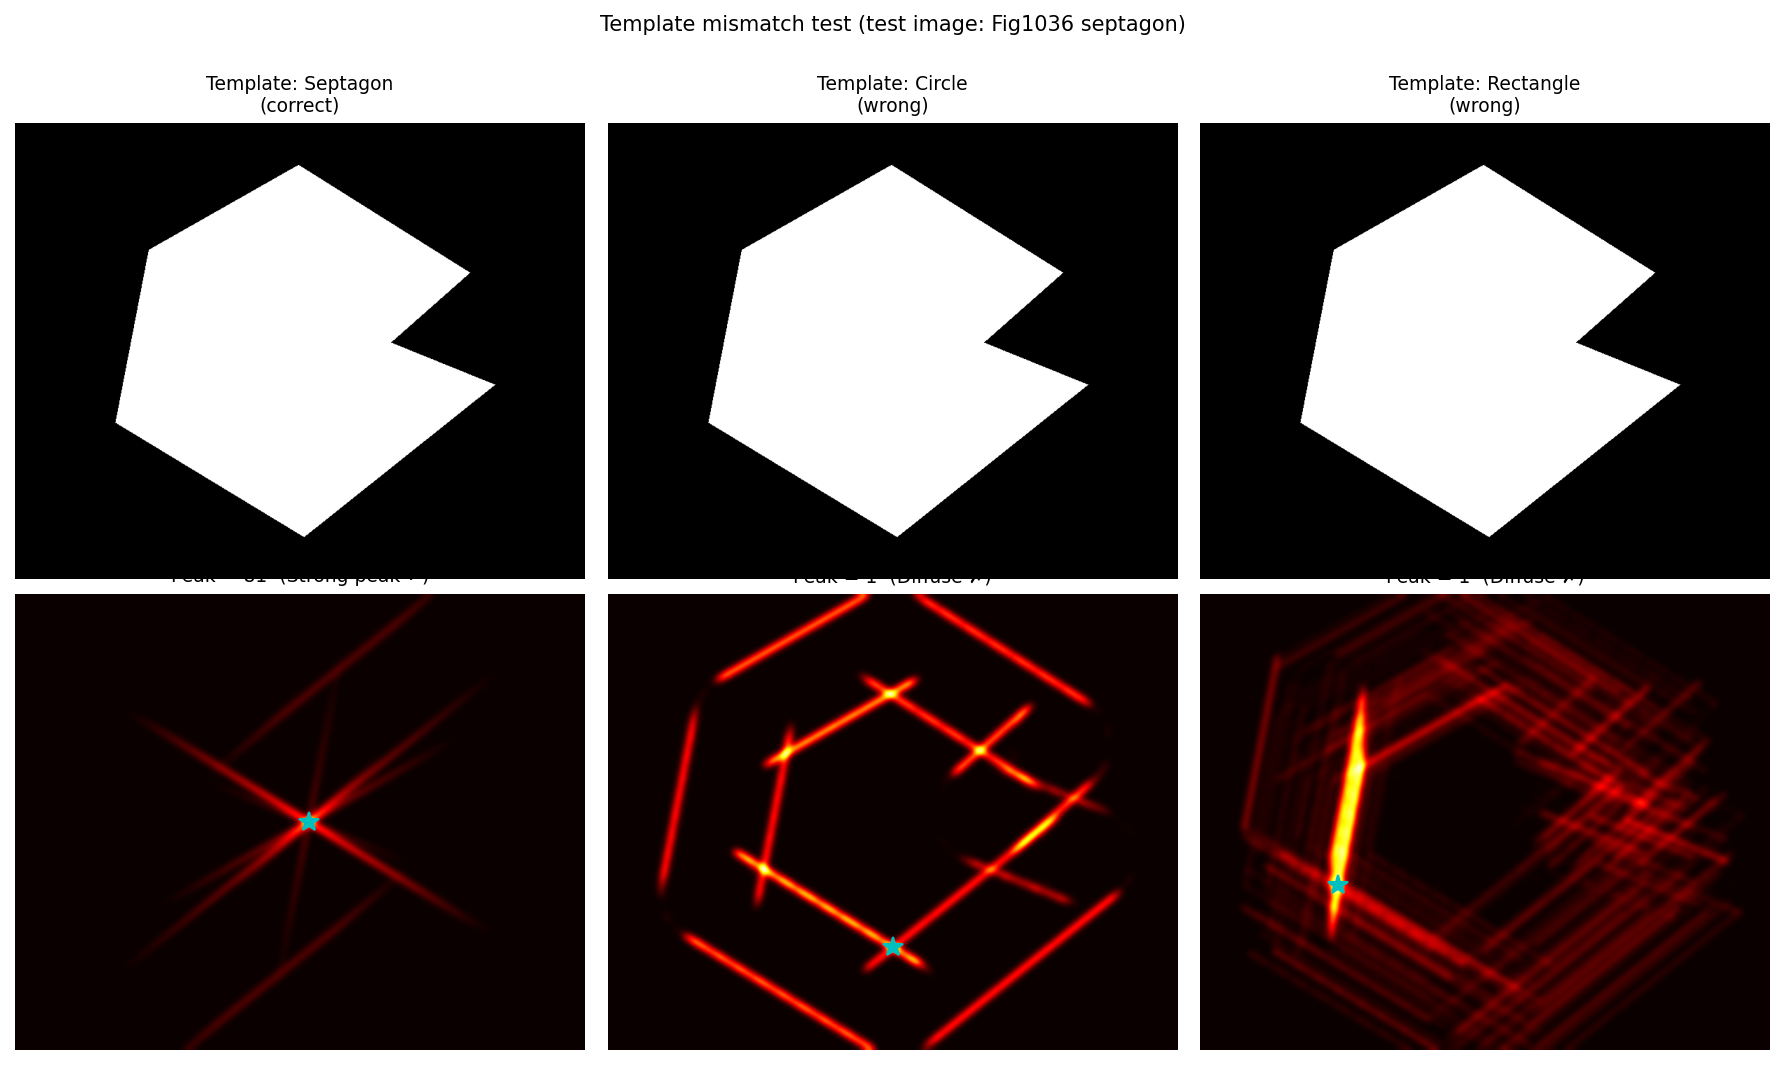
\includegraphics[width=0.85\textwidth]{figures/fig_template_mismatch.png}
  \caption{Template mismatch test.  Test image: \texttt{Fig1036} septagon.
  Left: correct septagon template leads to a strong, well-localised accumulator peak.
  Centre and right: wrong templates (circle and rectangle) result in diffused accumulators
  with no dominant maximum.}
  \label{fig:template_mismatch}
\end{figure}

With the correct template the accumulator is clearly dominated by a single peak.
With the circle or rectangle template the accumulator surface is comparatively
featureless. The vote counts are still nonzero, because some edge pixel
orientations happen to align partially by chance, but no location receives a
coherent contribution from the whole boundary at once.  

\subsection{Summary of Experimental Results}

\begin{table}[H]
\centering
\caption{Summary of all experimental results reported in this tutorial.}
\label{tab:summary}
\renewcommand{\arraystretch}{1.3}
\begin{tabular}{@{} l l p{3.6cm} p{4cm} @{}}
\toprule
\textbf{Image} & \textbf{Experiment} & \textbf{Challenge} & \textbf{Outcome} \\
\midrule
FigP0917 & Worked example    & Noisy binary boundary          & Exact detection, offset $(0,0)$ \\
Fig0941  & Multi-scale GHT   & Variable size, 48 instances    & All 48 dowels found \\
Fig1036  & Irregular polygon & Non-convex 7-sided shape       & Zero error; star-burst acc. \\
Fig0219  & Noise robustness  & $\sigma_n = 30$ additive noise & Peak survives; floor rises \\
FigP0917 & Partial occlusion & 0\%--70\% boundary removed     & Graceful linear degradation \\
FigP0917 & Scale mismatch    & $0.5\times$--$1.5\times$       & Peak collapses off-scale \\
Fig1036  & Rotation mismatch & $0^\circ$--$90^\circ$          & Peak collapses off-orientation \\
Fig1036  & Template mismatch & Wrong template applied         & Diffuse acc.; no false peak \\
\bottomrule
\end{tabular}
\end{table}

\subsection{Limitations}

The experiments above also expose the algorithm's practical constraints:
\begin{itemize}
  \item \textbf{Computational cost.}  The inner voting loop runs in
    $O(N_e \cdot K)$ time, where $K$ is the mean number of entries per R-table bin.
    For large, complex shapes or high-resolution images this can be slow; adding
    scale and rotation sweeps multiplies cost by $N_s$ and $N_\theta$ respectively.
  \item \textbf{Scale and rotation rigidity.}  Without the extended accumulator,
    even modest departures from the training geometry collapse the accumulator peak,
    as demonstrated in Sections~\ref{sec:analysis}.2 and~\ref{sec:analysis}.3.
  \item \textbf{Template dependence.}  A template that does not faithfully represent
    the shape's boundary characte produces no useful detection, regardless of how well the algorithm
    itself is tuned.
  \item \textbf{Memory growth.}  The 4-D accumulator $A[y][x][s][\theta]$ scales as
    $O(W \cdot H \cdot N_s \cdot N_\theta)$ and can become prohibitively large when
    fine-grained scale and rotation sampling is required.
  \item \textbf{Sensitivity to clutter.}  A background rich in edges elevates the
    accumulator floor uniformly. If clutter is dense enough, the true peak may not
    clear the detection threshold.
\end{itemize}

% ═════════════════════════════════════════════════════════════════════════════
\section{Conclusion}
\label{sec:conclusion}
% ═════════════════════════════════════════════════════════════════════════════

This tutorial explained Generalised Hough Transform of
Ballard~\cite{ballard1981} from first principles to experimental validation. Ballard's work of substituting an R-table for a parametric equation converts
a shape-specific problem into a general one. Any shape for which a prototype exists
can be detected using the identical pipeline of edge extraction, gradient orientation,
table lookup, accumulator voting, and peak finding.

The real-image experiments reinforced three key points.  First: applying the scale-extended
GHT to \texttt{Fig0941} lifted the
detection count from the handful achievable with a single-radius template to all 48
visible dowels across a $2.8\times$ size range.  Second, the septagon result
demonstrated that the detection overlay genuinely traces an arbitrary irregular
boundary, including a non-convex feature, in a way that no standard Hough
parameterisation could achieve.  Third, the controlled mismatch experiments exposed some areas where the algorithm's tolerance ends, such as scale and rotation offsets that push gradient
lookups systematically into the wrong bins, causing rapid collapse of the
accumulator peak, confirming that the extended accumulator described by
Ballard~\cite{ballard1981} is necessary whenever such transformations are expected.

The voting paradigm that underpins the GHT continues to influence modern
approaches, such as the Implicit Shape Models~\cite{leibe2004} generalise the same idea to
learned, part-based shape representation, and it remains a useful conceptual
framework for understanding why methods from Random Forests to Hough Forests work as
well as they do.

% ═════════════════════════════════════════════════════════════════════════════
\begin{thebibliography}{99}
% ═════════════════════════════════════════════════════════════════════════════

\bibitem{ballard1981}
D.~H. Ballard,
``Generalizing the Hough transform to detect arbitrary shapes,''
\textit{Pattern Recognition}, vol.~13, no.~2, pp.~111--122, 1981.

\bibitem{hough1962}
P.~V.~C. Hough,
``Method and means for recognizing complex patterns,''
U.S. Patent 3,069,654, 1962.

\bibitem{duda1972}
R.~O. Duda and P.~E. Hart,
``Use of the Hough transformation to detect lines and curves in pictures,''
\textit{Communications of the ACM}, vol.~15, no.~1, pp.~11--15, 1972.

\bibitem{merlin1975}
P.~M. Merlin and D.~J. Farber,
``A parallel mechanism for detecting curves in pictures,''
\textit{IEEE Trans. Computers}, vol.~C-24, no.~1, pp.~96--98, 1975.

\bibitem{canny1986}
J.~Canny,
``A computational approach to edge detection,''
\textit{IEEE Trans. Pattern Analysis and Machine Intelligence},
vol.~8, no.~6, pp.~679--698, 1986.

\bibitem{illingworth1988}
J.~Illingworth and J.~Kittler,
``A survey of the Hough transform,''
\textit{Computer Vision, Graphics, and Image Processing},
vol.~44, no.~1, pp.~87--116, 1988.

\bibitem{leibe2004}
B.~Leibe, A.~Leonardis, and B.~Schiele,
``Combined object categorization and segmentation with an implicit shape model,''
\textit{ECCV Workshop on Statistical Learning in Computer Vision}, 2004.

\bibitem{bradski2000}
G.~Bradski,
``The OpenCV library,''
\textit{Dr.\ Dobb's Journal of Software Tools}, 2000.

\bibitem{harris2020}
C.~R. Harris \textit{et al.},
``Array programming with NumPy,''
\textit{Nature}, vol.~585, pp.~357--362, 2020.

\bibitem{virtanen2020}
P.~Virtanen \textit{et al.},
``SciPy 1.0: Fundamental algorithms for scientific computing in Python,''
\textit{Nature Methods}, vol.~17, pp.~261--272, 2020.

\bibitem{gonzalez2018}
R.~C. Gonzalez and R.~E. Woods,
\textit{Digital Image Processing}, 4th~ed.
Pearson, 2018.

\bibitem{nixon2019}
M.~S. Nixon and A.~S. Aguado,
\textit{Feature Extraction and Image Processing for Computer Vision}, 4th~ed.
Academic Press, 2019.

\end{thebibliography}

\end{document}